\documentclass[11pt,a4paper]{article}
\usepackage{fontspec}
\setmainfont{Source Serif 4}[Path=/home/claude/ref/fonts/, UprightFont=SourceSerif4-Regular.ttf, BoldFont=SourceSerif4-Semibold.ttf, ItalicFont=SourceSerif4-It.ttf]
\setmonofont{IBM Plex Mono}[Path=/home/claude/ref/fonts/, UprightFont=IBMPlexMono-Regular.ttf, BoldFont=IBMPlexMono-Medium.ttf, Scale=0.88]
\usepackage[a4paper,margin=2.4cm]{geometry}
\usepackage{amsmath}
\usepackage{graphicx,booktabs,float,caption,array,xcolor,longtable}
\usepackage{xurl}
\usepackage[hidelinks]{hyperref}
\usepackage[round]{natbib}
\usepackage{setspace}
\setstretch{1.08}
\renewcommand{\topfraction}{0.9}
\renewcommand{\bottomfraction}{0.8}
\renewcommand{\textfraction}{0.1}
\renewcommand{\floatpagefraction}{0.75}
\setlength{\parindent}{0pt}
\setlength{\parskip}{0.55em}
\captionsetup{font=small,labelfont=bf}
\setlength{\bibsep}{3pt}
\urlstyle{same}
\hypersetup{pdftitle={The Trig Pillar Network},pdfauthor={Dr Tristan Hotham}}

\begin{document}
\begin{center}
{\Large\bfseries The Trig Pillar Network: Geometry, Construction, Survival and Intervisibility of the Ordnance Survey Retriangulation of Great Britain\par}
\vspace{1.2em}
{\large Dr Tristan Hotham\par}
\vspace{0.3em}
{\small Independent researcher\\
ORCID: 0000-0003-4931-9349\\
DOI: https://doi.org/10.5281/zenodo.24104644\par}
\vspace{0.8em}
2026
\end{center}

\begin{quote}
\small
\begin{center}\textbf{Abstract}\end{center}
The Retriangulation of Great Britain, begun in 1936, left thousands of concrete pillars on British hilltops and gave the country its National Grid. Treating the Ordnance Survey's legacy station list as data, this paper asks four questions, pre-specified in a written plan: how the network is laid out, when it was built, how much is recorded destroyed, and whether a modern open terrain model reproduces the rule that neighbouring stations of the same order must be intervisible. Grouping 31,521 mark records into 24,433 stations (6,573 pillars), I find a clear hierarchy of spacing (median nearest same-order distance 19.6 km for primary stations, 7.1 km for secondary and 4.3 km for third-order pillars), primaries far more regular than random points (Clark and Evans ratio 1.54 against 1.02 to 1.17), and 99.0\% of pillars dated 1936 to 1962. Over Terrain Tiles (zoom 9), with curvature and refraction, 228 of 240 nearest-neighbour primary lines are clear (95.0\%, 95\% CI 91.5 to 97.1), against 16.6\% when both ends are moved 1 km and 10.9\% for random land pairs of the same lengths. Of the 12 failures, 8 involve a structure without a recorded height and 3 a station observed from a steel tower; one is unexplained. The result depends on using surveyed station heights: with the terrain model's own heights at the ends, only 67.1\% of lines are clear, because the model sits a median 22 m below surveyed pillar tops. Pillars are far less often recorded destroyed (6.3\%) than other marks.

\textbf{Keywords:} triangulation; Ordnance Survey; geodetic networks; intervisibility; viewshed; digital elevation models; history of surveying
\end{quote}

\section{Introduction}\label{sec:intro}
Few objects of the twentieth century are as familiar in the British landscape, and as little studied as a population, as the triangulation pillar. The Ordnance Survey (OS) began the Retriangulation of Great Britain on 18 April 1936, when it first used a pillar, at Cold Ashby in Northamptonshire \citep{osblog2016}; the official history dates the project from 1935 \citep{os1967}. More than 6,500 pillars were built, to a design by Martin Hotine \citep{osblog2016}, and the network they carried was computed in seven blocks to define the OSGB36 datum on which the National Grid rests \citep{greaves2004,os1967}. Satellite positioning has since replaced triangulation as the way coordinates are fixed in Britain: since the OSTN02 transformation, the National Grid is defined by a transformation from GPS-derived coordinates rather than by the coordinates of the triangulation stations themselves \citep{greaves2004}. Yet the pillars remain, visited by walkers and logged by enthusiasts, and the OS still publishes the legacy list of its old stations.

That list has been used as a gazetteer but, as far as I can find, not as data about the network itself. The official history of the Retriangulation \citep{os1967} and the general histories of the OS \citep{seymour1980,owen1992} describe how the network was planned and observed. They do not, and could not at the time, measure the whole network as a spatial object: how regular it is, how its orders nest, how much of it survives, or whether the line-of-sight design that governed every station's siting can be recovered from a modern terrain model. This paper does those things, with four questions fixed in a written plan before the outcomes were computed (Section~\ref{sec:design}).

The fourth question is the main test. Triangulation needs every station to be visible from its neighbours, because angles are measured by sighting a theodolite on the next station's signal. If the station list is accurate and a modern open terrain model represents the land well enough, neighbouring stations of the same order should be intervisible over that model, once the curvature of the Earth and atmospheric refraction are allowed for. That prediction is not trivial: open global terrain models are coarse, they smooth summits, and they carry errors that are known to produce large uncertainty in visibility analysis \citep{fisher1991,fisher1993}. A high intervisibility rate would show that the terrain model reproduces the design; a low one would show the limits of the model, or of the list. Placebo lines, built from the same terrain at the same lengths but with the ends moved, separate the effect of the surveyors' siting from the general openness of British terrain.

The results are clear. The network is a nested, regular mesh. It was built in about a generation. Its pillars survive far better than its other marks. And 95\% of nearest-neighbour primary lines are clear over the terrain model, far above either placebo, with all but one of the failures explained by a missing structure height or by flat country where the surveyors observed from steel towers. That result depends on the surveyed station heights: with the terrain model's own heights at the ends, the share falls to 67\%, though it stays well above the placebos. The paper contributes a reproducible, open measurement of a national geodetic network, a validation of a widely used open terrain product at survey stations, and a simple template for testing intervisibility designs with open data.

\section{Background and literature}\label{sec:lit}
\subsection{From the Principal Triangulation to the Retriangulation}
British triangulation began with William Roy's measurement of the distance between the meridians of the Greenwich and Paris observatories, reported to the Royal Society in 1790 \citep{roy1790}. The Principal Triangulation of Great Britain that followed, observed between 1783 and 1853 \citep{osblog2016}, was published by \citet{clarke1858}; its early history is told by \citet{hewitt2010}, and its imperial counterpart in India by \citet{edney1997}. The Retriangulation was designed to replace it with a new, homogeneous network on a single national projection, the basis of the National Grid \citep{os1967,seymour1980,owen1992}.

The Retriangulation was observed between 1936 and 1953 and computed by hand in seven blocks, with scale and orientation held to eleven stations of the Principal Triangulation \citep{greaves2004}. The resulting datum, OSGB36, is internally inconsistent at the level of metres: \citet{greaves2004} reports that the National Grid is about 20 m too long over the length of Great Britain. The network was later readjusted \citep{ashkenazi1972} and, in OS(SN)80, readjusted together with the triangulation of Ireland \citep{ashkenazi1983}, but OSGB36 remained the mapping datum \citep{greaves2004}. The secondary, third-order and fourth-order networks filled the primary triangles, down to bolts on buildings and intersected points such as church spires \citep{seymour1980,owen1992}.

The pillar itself was the Retriangulation's main physical innovation: a concrete or stone column 1.2 m high with a brass plate on top to take the survey instrument, giving a stable, reoccupiable station (in the OS's description of its station types, quoted by \citealt{jones2018}). Where pillars were impractical, in difficult terrain from about 1958, a lighter cylindrical design (the ``Vanessa'') was used \citep{tukpillar}. In flat country, where trees and buildings blocked lines at ground level, observers raised the theodolite on steel Bilby towers, commonly about 100 ft (30 m) high: the TrigpointingUK wiki, citing the OS history and \citet{owen1992}, lists 22 primary stations, mostly in eastern England and built in 1938 and 1939, where such towers were used \citep{tukbilby}. This detail matters below.

\subsection{Spatial structure of point networks}
Two classic tools describe how regular a set of points is. The nearest-neighbour statistic of \citet{clarkevans1954} compares the mean distance from each point to its nearest neighbour with the value expected for complete spatial randomness (CSR); ratios above 1 indicate regularity. \citet{ripley1977} developed the wider theory of point-pattern models and tests, and \citet{baddeley2015} give a modern treatment, including the edge effects that bias the simple ratio near a boundary such as a coastline. Monte Carlo simulation of CSR within the same window is the standard remedy and is used here. Triangle shape is a second, survey-specific measure: well-conditioned triangles, with no very small angle, propagate angular errors less badly into positions. The Delaunay triangulation \citep{delaunay1934}, here computed with the Quickhull algorithm \citep{barber1996} as implemented in SciPy \citep{virtanen2020}, gives a canonical net of neighbouring triangles for any point set.

\subsection{Visibility analysis and terrain models}
Line-of-sight and viewshed analysis are long-standing GIS operations. \citet{lee1991} framed visibility site selection on terrain as a problem in its own right, with military surveillance and the siting of radio transmitters among its applications, and \citet{defloriani1994} reviewed algorithms for point, line and region visibility on terrain models. \citet{kim2004} explored choosing several observer sites to maximise joint visibility, the modern version of the surveyor's siting problem. A strong theme of this literature is uncertainty: \citet{fisher1991} showed that adding plausible elevation error to a terrain model changes viewshed areas, so that the viewshed computed from the original model may substantially overestimate the visible area, and \citet{fisher1993} found that the representation of viewpoint and target in different algorithms changed the visible area by up to 50\% above the mean. The resolution of the terrain model matters too: \citet{zhang1994} showed that grid size substantially changes the terrain parameters computed from a model. Long sight lines must also allow for the curvature of the Earth and for refraction. The conventional coefficient of refraction for geodetic work is about 0.13, but \citet{hirt2010} measured it near the ground and found it varied widely, from about $-4$ to $+16$ on sunny days, and concluded that the conventional value is unsuitable close to the ground. Here the lines run between hilltops and the coefficient is varied as a robustness check.

The terrain model used here is Terrain Tiles, an open, global tiled elevation product built by Mapzen and hosted on AWS Open Data. At zoom 9 its land elevations come mainly from SRTM \citep{farr2007} and, in Europe, EU-DEM, with GMTED2010 \citep{danielson2011} at high latitudes and ETOPO1 \citep{amante2009} for bathymetry \citep{tilezen}. Its pixels are about 190 m across at British latitudes.

\subsection{What is new here}
Histories of the Retriangulation describe its design; geodetic studies analyse its observations and adjustments; visibility research tests algorithms on terrain. None, as far as I can find, measures the whole network from the legacy station list, or tests the network's defining design rule against an open terrain model with placebo lines. The paper offers three things: a cleaned, station-level version of the legacy list with order, kind, date and survival; measurements of spacing, regularity, triangle shape, construction and survival with uncertainty; and an intervisibility test that validates both the list and the terrain model, with the failures read one by one.

\section{Data}\label{sec:data}
\subsection{The OS legacy triangulation station list}
The OS published a list of its legacy triangulation stations; \citet{jones2018} packaged it as the R package trigpoints (package code under the MIT licence; ``Contains OS data \textcopyright\ Crown copyright and database right 2018''). The OS has stated that the station data may be used under the Open Government Licence v3.0, under which the derived station table is redistributed with this paper. The package notes that the list is no longer maintained by the OS, so stations marked as not destroyed may no longer exist, and that its coordinates are expected to be accurate to within about a metre of OSGB36. The list has 31,521 rows. Each row is a mark, not a station: one station can have a pillar, a bolt beneath it, a centre mark and a refixed mark. Fields include the name, station code, order (1 to 4, plus a few later codes), type of mark, height, commissioning date, destroyed flag, notes and easting and northing.

\subsection{From marks to stations}
Rows sharing a station code within 100 m were grouped into one station (some codes are placeholders reused across the country, such as those of 1990s GPS stations, and these became separate stations by location). 2 exact duplicate rows were dropped. This gives 24,433 stations, with up to 11 rows each. A station is a pillar if any of its rows is a pillar; otherwise its kind is that of its main row, grouped into ground marks (bolts, rivets, blocks, buried blocks, centres and similar) and intersected or roof stations (spires, flagstaffs, vanes, chimneys, masts, lighthouses, towers and similar). Its order is the lowest of its rows; its commissioning year is the earliest; it is recorded destroyed if every row is flagged destroyed. Table~\ref{tab:stations} summarises the result: 6,573 pillars, of which 290 are primary, 2,130 secondary, 3,972 third order and 180 fourth order. The highest pillar in the list is Ben Nevis (1347 m).

\begin{table}[tbp]\centering\small\caption{Stations in the OS legacy list after grouping mark rows, by order and kind, with the share recorded destroyed.}\label{tab:stations}\begin{tabular}{lrrrrr}\toprule Order & Pillars & Ground marks & Intersected & All & Destroyed (\%)\\\midrule
Primary (1) & 290 & 50 & 7 & 347 & 8.6\\
Secondary (2) & 2,130 & 668 & 140 & 2,938 & 9.4\\
Third order (3) & 3,972 & 4,155 & 3,508 & 11,635 & 20.4\\
Fourth order (4) & 180 & 7,113 & 2,119 & 9,412 & 38.3\\
Later codes & 1 & 100 & 0 & 101 & 7.9\\
\midrule All & 6,573 & 12,086 & 5,774 & 24,433 & 25.8\\
\bottomrule\end{tabular}\end{table}

Stations were placed in an ONS region of England, or in Scotland or Wales, by point in polygon; 463 stations on rocks, piers and lighthouses outside the land polygons were assigned the nearest region. Coordinates were converted to latitude and longitude with pyproj (EPSG:27700 to EPSG:4326).

\subsection{Terrain}
Terrain Tiles at zoom 9 (Terrarium encoding) covering Great Britain and Ireland were mosaicked and sampled with bilinear interpolation. The mosaic's western edge lies at 8.44 degrees west, so 11 stations of the St Kilda group, including the primary station St Kilda, have no terrain value. They are kept in the geometry and survival analyses and treated as sea along their lines of sight, where the profile is open water.

\subsection{OpenStreetMap survey points}
For an independent check on survival, I used the 2,909 survey points in the UK from OpenStreetMap (ODbL), retrieved in 2026 through the QLever query service. Only 299 are tagged as pillars, and coverage of trig points in this extract is clearly partial, so the OSM data serve only as a check, not as a census.

\section{Research design}\label{sec:design}
\subsection{Analysis plan}
The plan, with hypotheses, measures, decision rules and robustness checks, was written in the study's notes (NOTES.md, released with the data) after the data had been profiled descriptively and before any spacing statistic, intervisibility result or survival rate was computed. It is summarised here; anything added later is labelled exploratory.

\subsection{Q1: geometry}
For each order, the distance from each station to its nearest station of the same order was computed, for all kinds of station in order 1 and for pillars in orders 2 and 3. Medians carry bootstrap 95\% intervals \citep{efron1979}. \textbf{H1} predicts that the median falls with order. The Clark and Evans ratio $R = \bar d / (0.5/\sqrt{\lambda})$, with $\lambda$ the number of stations per km$^2$ of land, was compared with 199 CSR simulations of the same number of points on the same land mask (49 for the largest sets), which carry the same coastal edge effect. \textbf{H2} predicts $R$ above the CSR band for primaries. Primary stations were joined by a Delaunay triangulation; triangles with any side over 80 km or a centroid more than 10 km from land were dropped. The share of triangles whose every angle is at least 30 degrees was compared with the same share for CSR points.

\subsection{Q2: construction}
Commissioning years are summarised by order and kind. \textbf{H4} predicts that at least 75\% of pillars are dated 1936 to 1962. Many primary stations carry the date of their block of the network rather than their own, so the year is read as an approximate build date.

\subsection{Q3: survival}
The destroyed flag is summarised by kind, order and region with Wilson intervals \citep{wilson1927}. The main model is a logit of the destroyed flag on kind, order, region, lowland (terrain model height below 100 m) and decade of commissioning, with standard errors clustered by 10 km grid square \citep{cameron2015}, estimated with statsmodels \citep{seabold2010}. \textbf{H5} predicts lower odds for pillars than for intersected stations and ground marks, and higher odds in the lowlands.

\subsection{Q4: intervisibility}
\textbf{Lines.} For every primary station, the line to its nearest primary neighbour; for every secondary and third-order pillar, the line to its nearest pillar of the same order; unique undirected pairs. As a secondary set, every side of the primary Delaunay net up to 80 km.

\textbf{Heights.} Each end is placed at the station's recorded height where one is given (the OS height of the mark), otherwise at the terrain model's height, plus 1.5 m for the instrument or signal.

\textbf{Profile.} The terrain is sampled every 100 m along the straight line in the National Grid. Each sample is lowered by $d_1 d_2 (1-k)/(2R)$, where $d_1$ and $d_2$ are the distances to the two ends, $R = 6{,}371$ km and the refraction coefficient $k = 0.13$; sea and missing values are set to zero. The line is clear if no sample, ignoring those within 250 m of either end (about one terrain pixel), rises above it. The minimum clearance in metres is recorded.

\textbf{Hypothesis and decision rule.} \textbf{H3} predicts that at least 80\% of nearest-neighbour primary lines are clear; it would count against H3 if the lower bound of the Wilson 95\% interval fell below 80\%.

\textbf{Placebos.} (a) The same lines with each end moved 1 km in a random direction onto land, at ground level plus 1.5 m (ten draws per line); this asks whether exact siting matters. (b) Random pairs of land points with the same lengths and random bearings (ten draws per line). Differences in share carry bootstrap intervals.

\textbf{Robustness.} Refraction $k = 0$, 0.075 and 0.20; end margins of 0 and 500 m; instrument heights of 0 and 5 m; a 50 m profile step; the two nearest neighbours instead of one; terrain-model heights at both ends instead of surveyed heights; pillar-to-pillar lines only; and leaving out each region in turn.

\textbf{Validation.} The terrain model's height at each pillar with a recorded height is compared with that height. Every failing primary line is read by eye from its profile.

\section{Results}\label{sec:results}
\subsection{Geometry}
H1 is supported (Table~\ref{tab:spacing}, Figure~\ref{fig:spacing}). The median distance from a primary station to its nearest primary neighbour is 19.6 km (95\% CI 18.5 to 20.6; interquartile range 13.1 to 25.6). For secondary pillars it is 7.1 km and for third-order pillars 4.3 km, with intervals that do not overlap. The sides of the primary Delaunay net have a median of 32.1 km (quartiles 22.8 to 42.3), longer than nearest-neighbour distances as expected, since each station's nearest neighbour is its shortest side.

\begin{table}[tbp]\centering\footnotesize\caption{Nearest same-order neighbour distances (km; median with bootstrap 95\% CI, interquartile range), density per 1,000 km$^2$ of land, and the Clark and Evans ratio with the 95\% band of CSR simulations on the same land.}\label{tab:spacing}\setlength{\tabcolsep}{2.5pt}\begin{tabular}{lrlllrl}\toprule Set & N & Median [95\% CI] & IQR & Density & $R$ & CSR band\\\midrule
Primary, all kinds & 347 & 19.62 [18.55, 20.59] & 13.14 to 25.61 & 1.5 & 1.54 & 1.02 to 1.17\\
Primary pillars & 290 & 20.97 [19.90, 22.01] & 15.06 to 27.02 & 1.3 & 1.54 & 1.03 to 1.18\\
Secondary, all kinds & 2,938 & 6.57 [6.46, 6.63] & 4.97 to 8.06 & 12.8 & 1.46 & 1.03 to 1.06\\
Secondary pillars & 2,130 & 7.09 [6.93, 7.21] & 5.54 to 8.63 & 9.3 & 1.39 & 1.02 to 1.08\\
Third order, all kinds & 11,635 & 2.07 [2.01, 2.14] & 0.99 to 3.56 & 50.6 & 1.08 & 1.02 to 1.04\\
Third-order pillars & 3,972 & 4.26 [4.22, 4.30] & 3.38 to 5.26 & 17.3 & 1.17 & 1.02 to 1.06\\
Fourth order, all kinds & 9,412 & 1.14 [1.12, 1.15] & 0.80 to 1.54 & 40.9 & 0.57 & 1.02 to 1.04\\
\bottomrule\end{tabular}\end{table}

\begin{figure}[tbp]\centering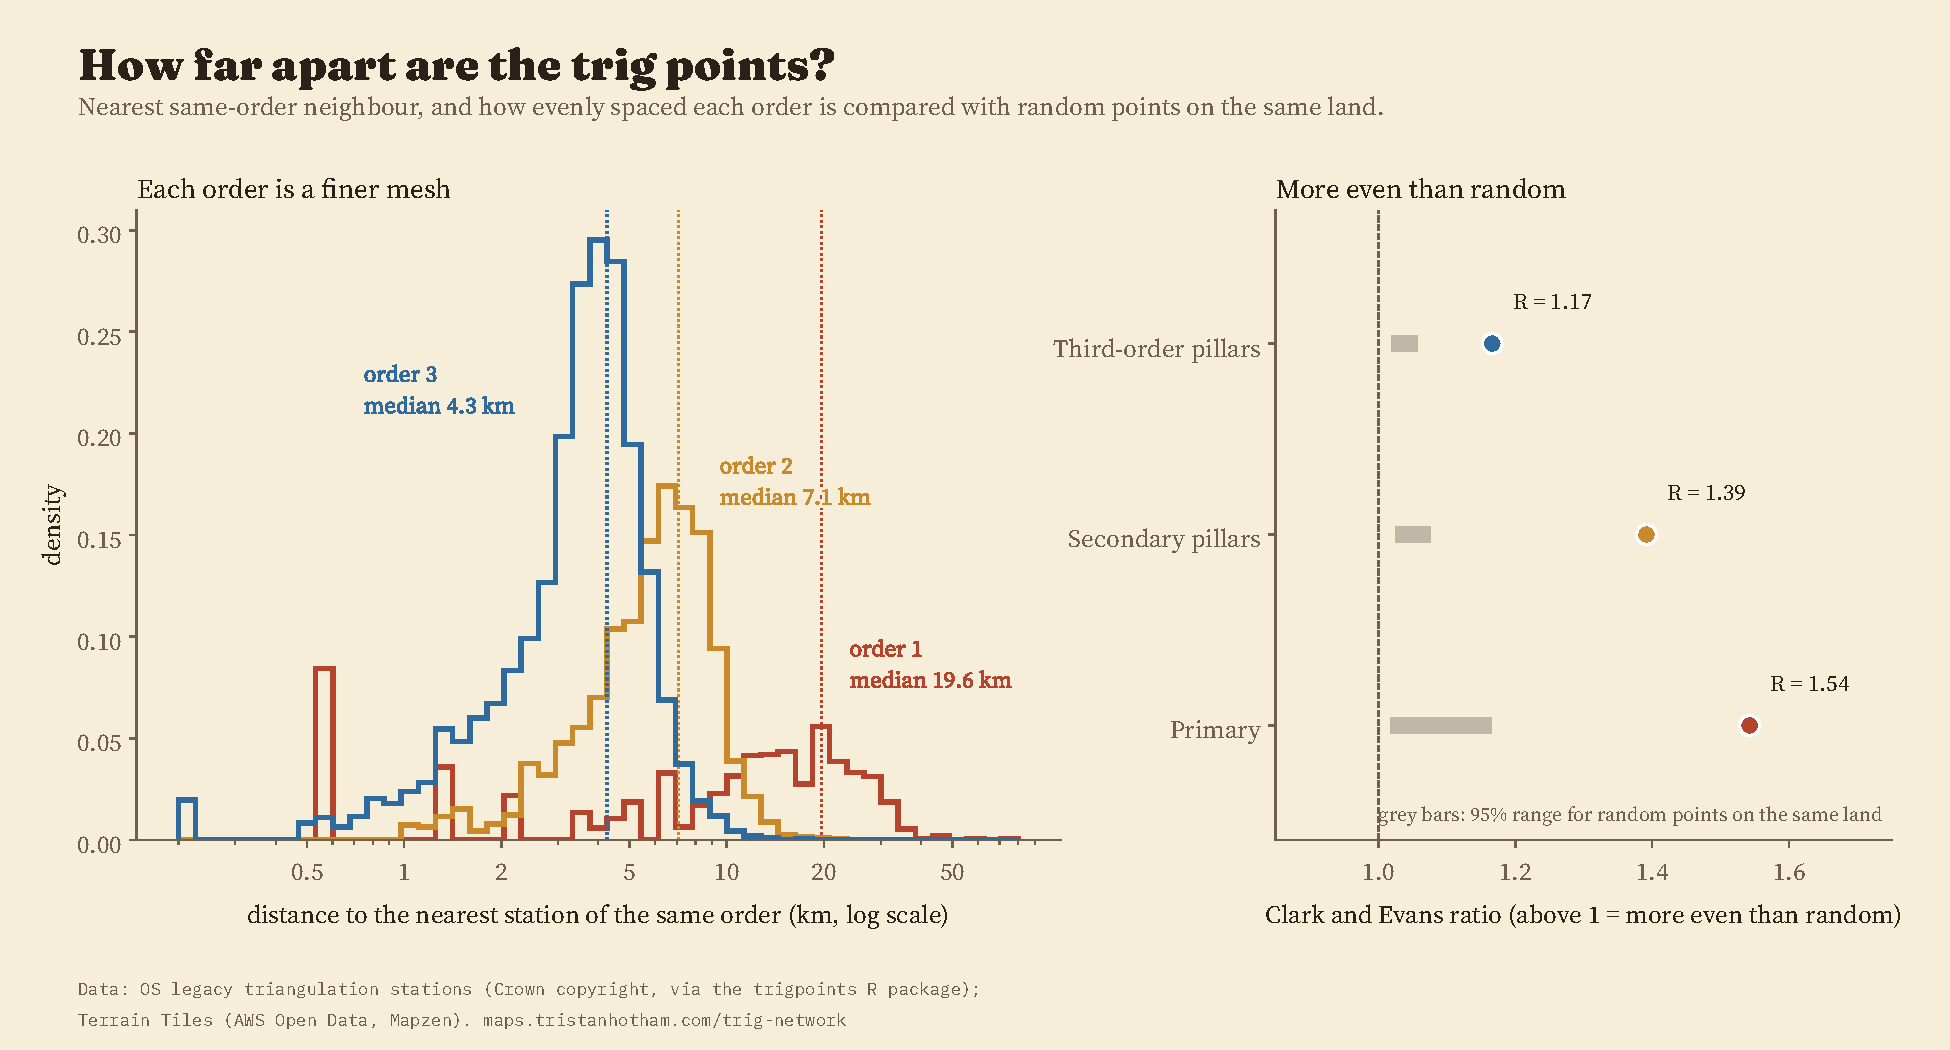
\includegraphics[width=\textwidth]{f_spacing.pdf}\caption{Nearest same-order neighbour distances (left) and the Clark and Evans ratio against 95\% bands from CSR simulations on the same land (right).}\label{fig:spacing}\end{figure}

H2 is supported. The Clark and Evans ratio for primaries is 1.54, well above the CSR band (1.02 to 1.17; none of 199 simulations as high, $p = 0.005$). Secondary pillars (1.39) and third-order pillars (1.17) are also more regular than random, the latter less so, as infill around towns and existing marks would lead one to expect. Fourth-order stations taken together are clustered rather than regular (ratio 0.57), consistent with their role as dense control in built-up areas. Of the 582 primary triangles, 71.3\% (bootstrap CI 67.5 to 74.9) have every angle of at least 30 degrees, against 48.0\% (95\% simulation band 43.7 to 51.9) for Delaunay triangles of random points (Figure~\ref{fig:triangles}). The median smallest angle is 35.9 degrees, against 29.2 for random points.

\begin{figure}[tbp]\centering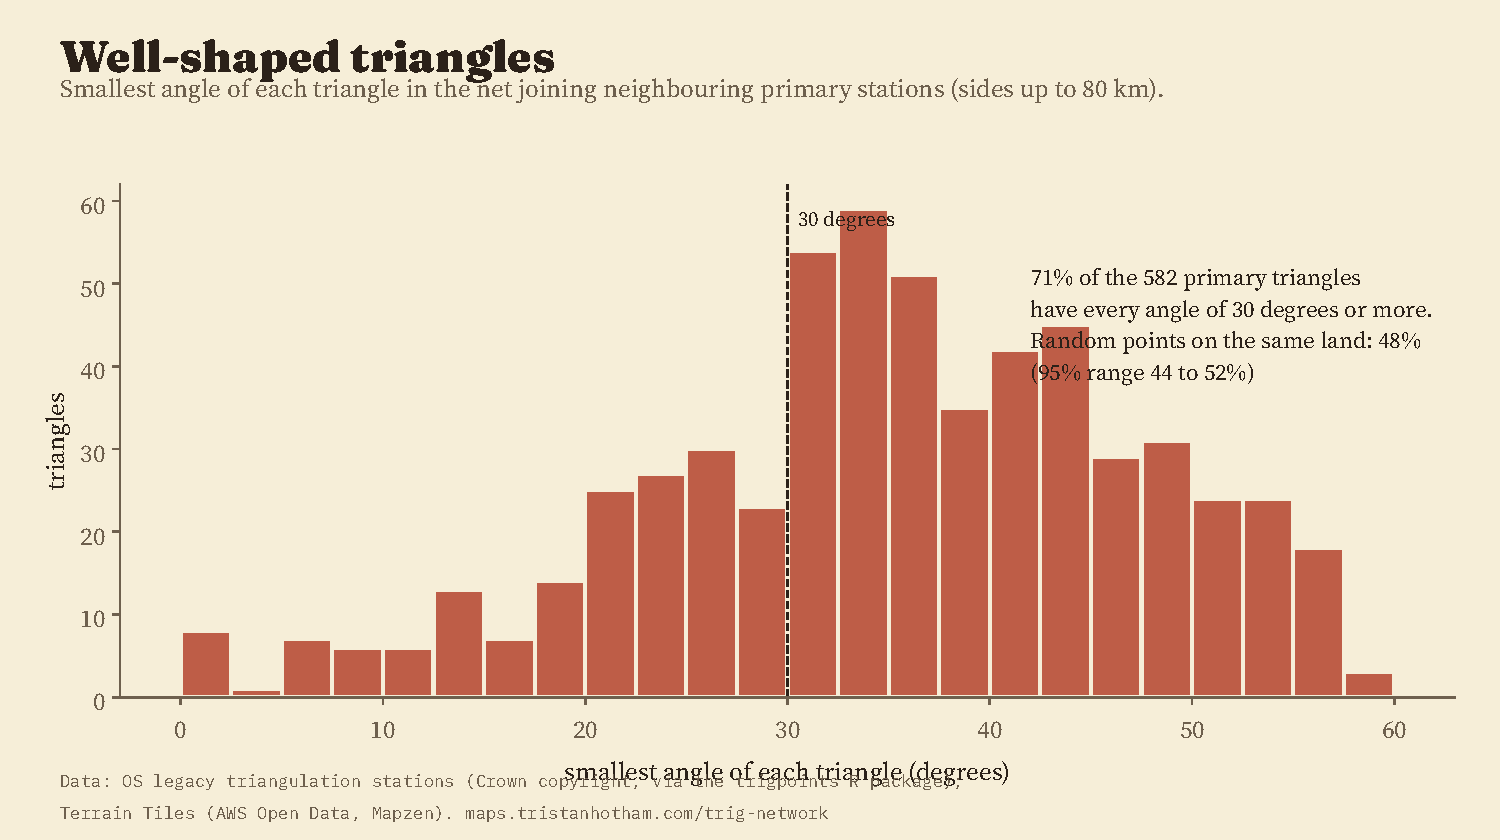
\includegraphics[width=0.85\textwidth]{f_triangles.pdf}\caption{Smallest angle of each primary Delaunay triangle (sides up to 80 km).}\label{fig:triangles}\end{figure}

\subsection{Construction}
H4 is supported (Figure~\ref{fig:build}). Of 6,573 pillars, 6,510 (99.0\%, Wilson CI 98.8 to 99.3) are dated 1936 to 1962. 604 pillars are dated 1936 to 1939, mostly primaries; none is dated 1940 or 1941; 2,316 are dated in the 1940s and 3,240 in the 1950s; the busiest single year is 1948 (744 pillars). Only 63 pillars are dated after 1962. The primary stations carry block dates: the six main figures are dated 1936 (FIG1 and FIG2), 1937 (FIG3 and FIG4), 1938 (FIG5) and 1951 (FIG6), with a small seventh figure dated 1952, which fits the account of primary work reaching northern Scotland only after the war \citep{greaves2004,os1967}.

\begin{figure}[tbp]\centering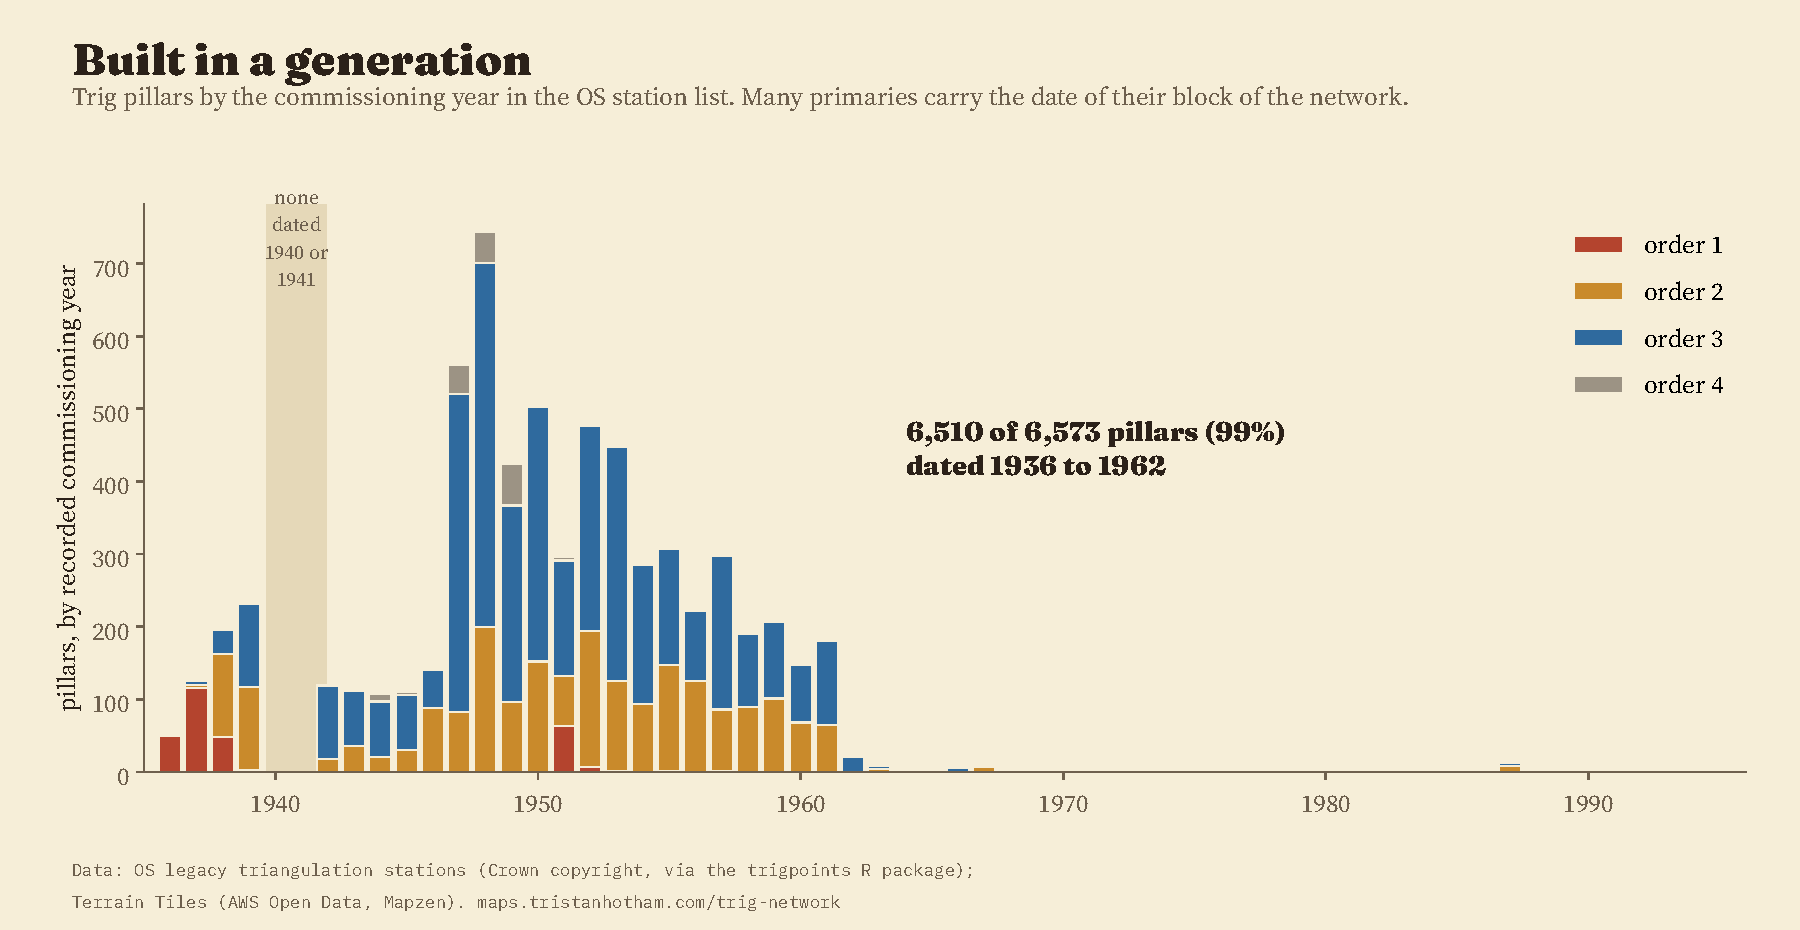
\includegraphics[width=\textwidth]{f_build.pdf}\caption{Pillars by commissioning year in the OS list, by order.}\label{fig:build}\end{figure}

\subsection{Intervisibility}
H3 is supported (Table~\ref{tab:vis}, Figures~\ref{fig:map} and~\ref{fig:vis}). Of the 240 nearest-neighbour primary lines (median length 20.2 km), 228 are clear over the terrain model: 95.0\% (Wilson CI 91.5 to 97.1), with a median clearance of 27 m. The lower bound is above the planned 80\% threshold. Of the 953 sides of the primary Delaunay net up to 80 km (median 33.0 km), 95.6\% are clear. Secondary pillars (97.1\% of 1,485 lines) and third-order pillars (91.9\% of 2,788) are similar; these were planned as exploratory.

\begin{table}[tbp]\centering\small\caption{Lines clear over the terrain model (Wilson 95\% CI). Main specification: surveyed heights plus 1.5 m, $k = 0.13$, 100 m step, 250 m end margin.}\label{tab:vis}\begin{tabular}{lrrl}\toprule Set & Clear & Lines & \% clear [95\% CI]\\\midrule
Primary, nearest neighbour (main) & 228 & 240 & 95.0 [91.5, 97.1]\\
Primary, Delaunay sides up to 80 km & 911 & 953 & 95.6 [94.1, 96.7]\\
\quad sides under 20 km & 151 & 170 & 88.8 [83.2, 92.7]\\
\quad sides 20 to 40 km & 450 & 465 & 96.8 [94.7, 98.0]\\
\quad sides 40 to 80 km & 310 & 318 & 97.5 [95.1, 98.7]\\
Secondary pillars, nearest neighbour & 1,442 & 1,485 & 97.1 [96.1, 97.8]\\
Third-order pillars, nearest neighbour & 2,562 & 2,788 & 91.9 [90.8, 92.9]\\
\midrule\multicolumn{4}{l}{\textit{Placebos (ground height plus 1.5 m at each end)}}\\
Primary lines, both ends moved 1 km & 399 & 2,400 & 16.6 [15.2, 18.2]\\
Random land pairs, primary lengths & 261 & 2,400 & 10.9 [9.7, 12.2]\\
Random land pairs, secondary lengths & 563 & 2,970 & 19.0 [17.6, 20.4]\\
Random land pairs, third-order lengths & 1,474 & 5,576 & 26.4 [25.3, 27.6]\\
\bottomrule\end{tabular}\end{table}

\begin{figure}[tbp]\centering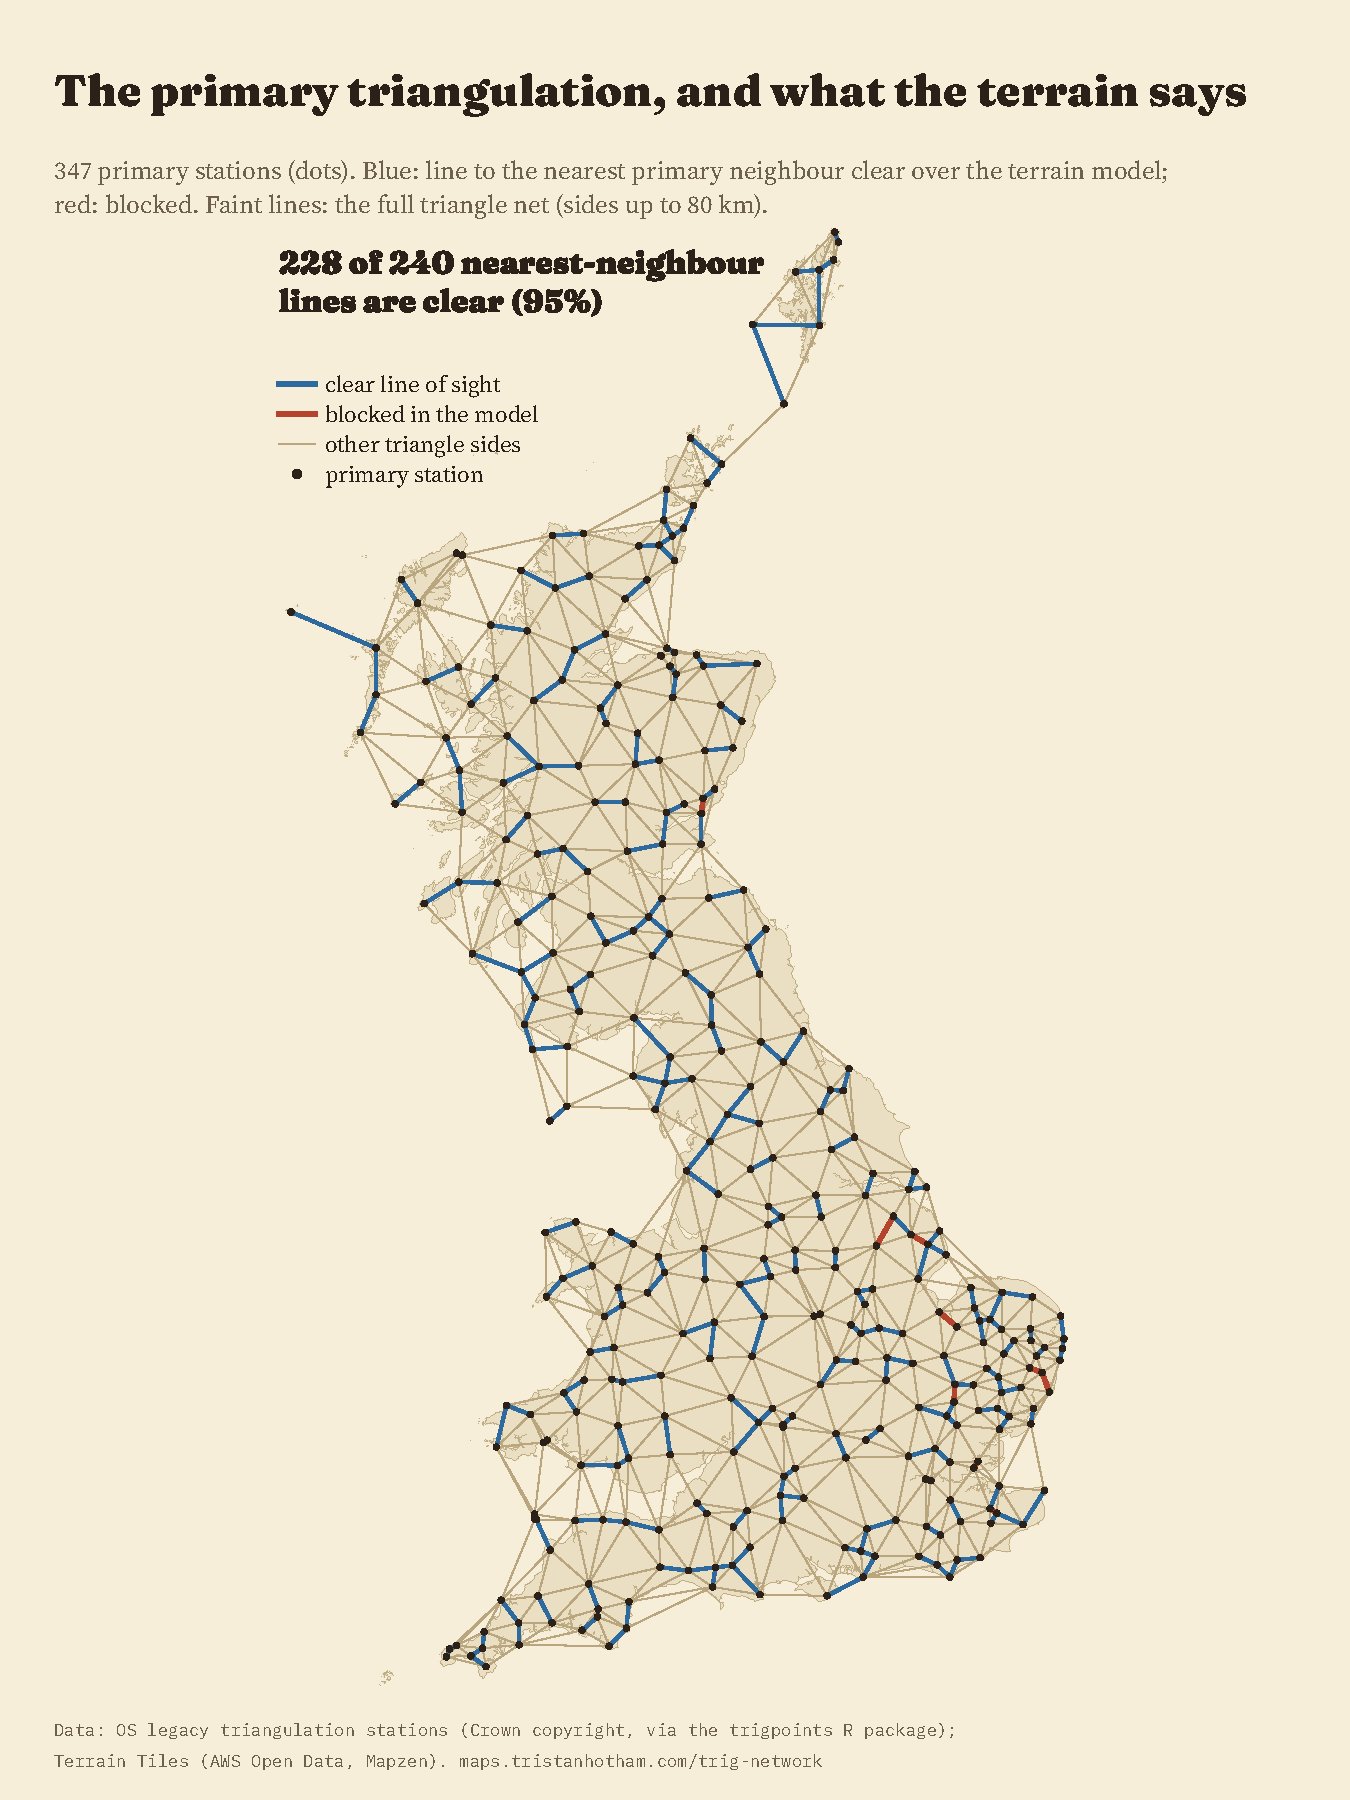
\includegraphics[width=0.72\textwidth]{f_map.pdf}\caption{The primary network: nearest-neighbour lines clear (blue) or blocked (red) over the terrain model, with the Delaunay net (faint).}\label{fig:map}\end{figure}

The placebos show how unusual this is. With both ends moved 1 km in a random direction, only 16.6\% of the same lines are clear; random land pairs with the same lengths are clear 10.9\% of the time. The differences are 78.4 percentage points (bootstrap CI 75.0 to 81.3) and 84.1 points (80.8 to 87.1). For secondary and third-order pillars, random land pairs of the same lengths are clear 19.0\% and 26.4\% of the time.

\begin{figure}[tbp]\centering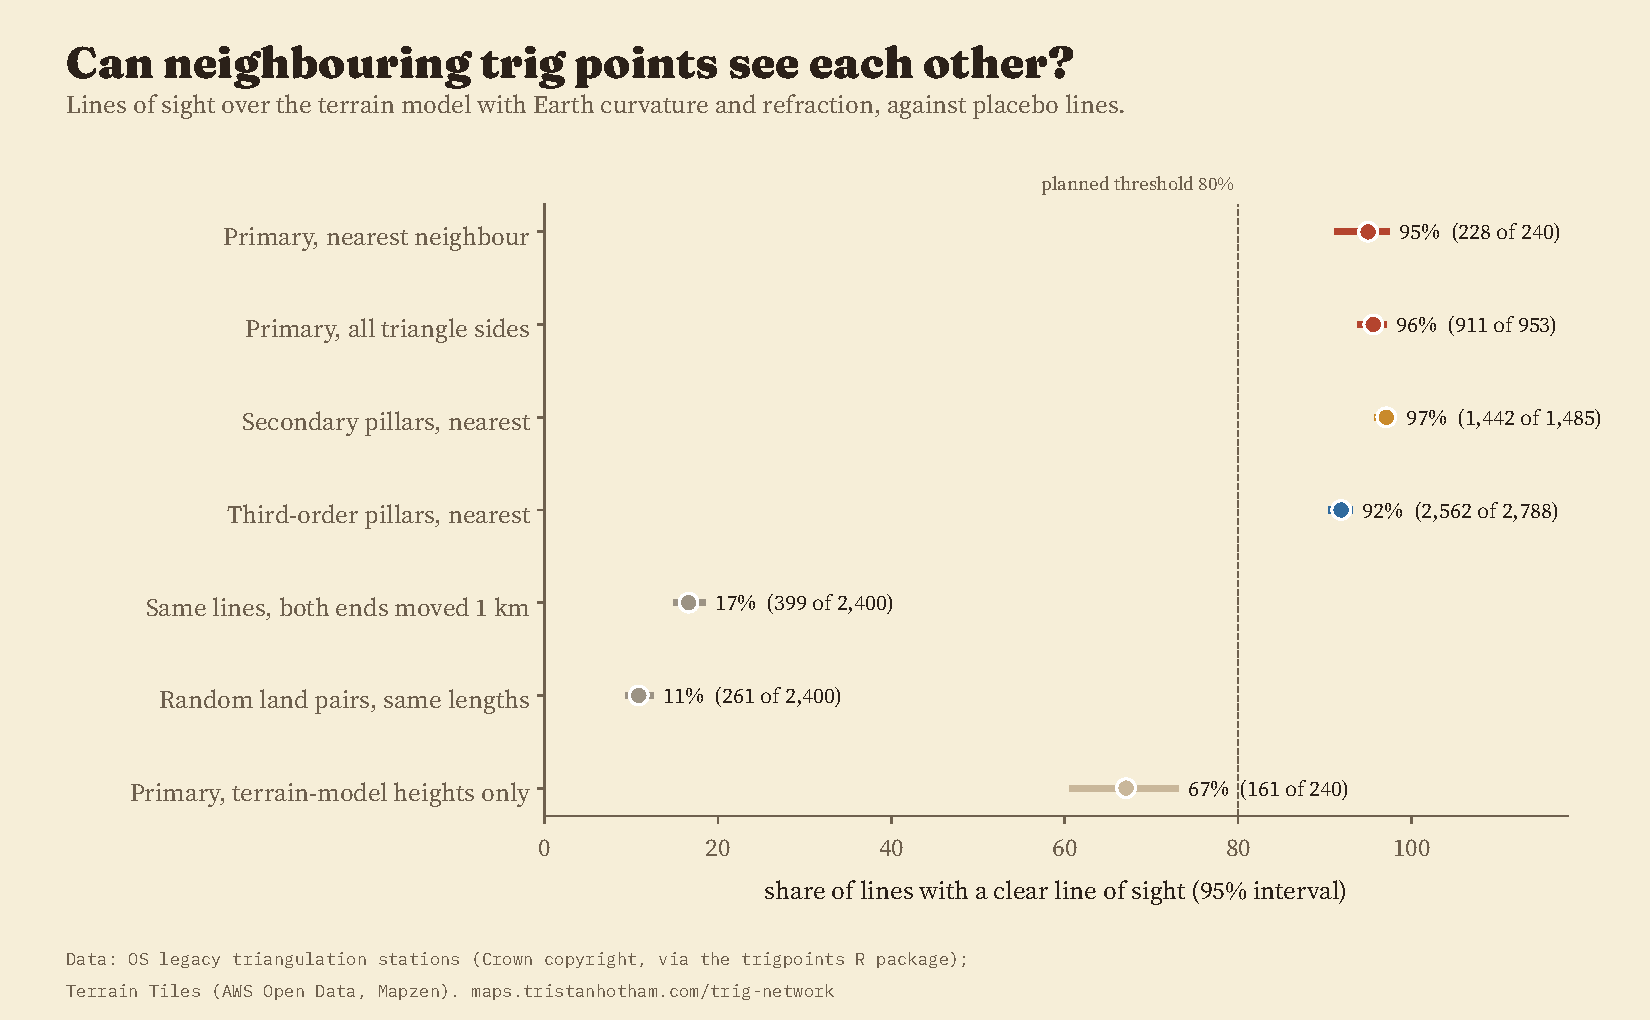
\includegraphics[width=\textwidth]{f_vis.pdf}\caption{Share of lines clear over the terrain model, with Wilson 95\% intervals, for the station sets and the placebos.}\label{fig:vis}\end{figure}

\subsection{The failures, one by one}
All 12 failing primary lines were read from their profiles (Table~\ref{tab:fail}; examples in Figure~\ref{fig:profiles}). 8 involve a station on a structure whose height the list does not record: the two Lundy lighthouse lines, Lincoln Minster, the Greenwich Observatory, Severndroog Castle, Orford Castle, and water towers at Lenham, Benfleet, Hockley and Burrough Green. For these the test puts the observer 1.5 m above the terrain model's ground, which misses the tower, spire or lantern that made the station useful; the profiles show shortfalls of a few metres to a few tens of metres, less than the height of such structures. One failure is not explained: West Hills to Buddon, where Buddon is a ground mark on the Tay coast with no recorded height and the line is blocked by 33 m of rising ground in the terrain model; the list's only note for Buddon reads ``Locating Coords'', and the data do not show how the line was observed. The remaining 3 failures are pillar-to-pillar lines in flat country (Salle to Crown Corner in Suffolk and Norfolk, Dexthorpe to Cold Harbour in Lincolnshire, Crimplesham to Walpole St Peters in Norfolk), blocked by between 1 and 3 m. Each has an end at one of the 22 primary stations listed as observed from a steel tower \citep{tukbilby}. As an exploratory check, raising the tower end to 30 m (about 100 ft) clears 3 of 3. Of the 27 nearest-neighbour primary lines touching a tower station, 24 are clear even at ground level, because the terrain model has no trees or buildings.

\begin{table}[tbp]\centering\footnotesize\caption{Every failing nearest-neighbour primary line: kinds of station (P pillar, G ground mark, I intersected or roof station), length (km), clearance (m; negative = blocked) and whether an end is a listed steel-tower station.}\label{tab:fail}\begin{tabular}{lllrrl}\toprule From & To & Kinds & km & Clearance & Tower\\\midrule
Lundy Island L Ho & Rat Island L Ho & I, I & 1.4 & $-$40.0 & \\
West Hills & Buddon & P, G & 12.7 & $-$32.6 & \\
Lundy Island L Ho & Lundy Island N W Point L Ho & I, I & 3.9 & $-$30.7 & \\
Benfleet Wtr Twr & Hockley Wtr Twr & G, G & 6.5 & $-$9.7 & \\
Lenham Wtr Twr & Frittenfield & I, G & 6.8 & $-$7.3 & \\
Acre & Lincoln Minster & P, G & 28.5 & $-$4.5 & \\
Dexthorpe & Cold Harbour & P, P & 16.3 & $-$3.1 & yes\\
Severndroog Castle & Greenwich Observatory & G, G & 4.4 & $-$3.0 & \\
Crimplesham & Walpole St Peters & P, P & 19.2 & $-$2.0 & yes\\
Orford Castle & Salle & G, P & 17.5 & $-$1.0 & \\
Salle & Crown Corner & P, P & 11.1 & $-$1.0 & yes\\
Burrough Green Wtr Twr & Helion Bumpstead & G, P & 14.8 & $-$0.6 & \\
\bottomrule\end{tabular}\end{table}

\begin{figure}[tbp]\centering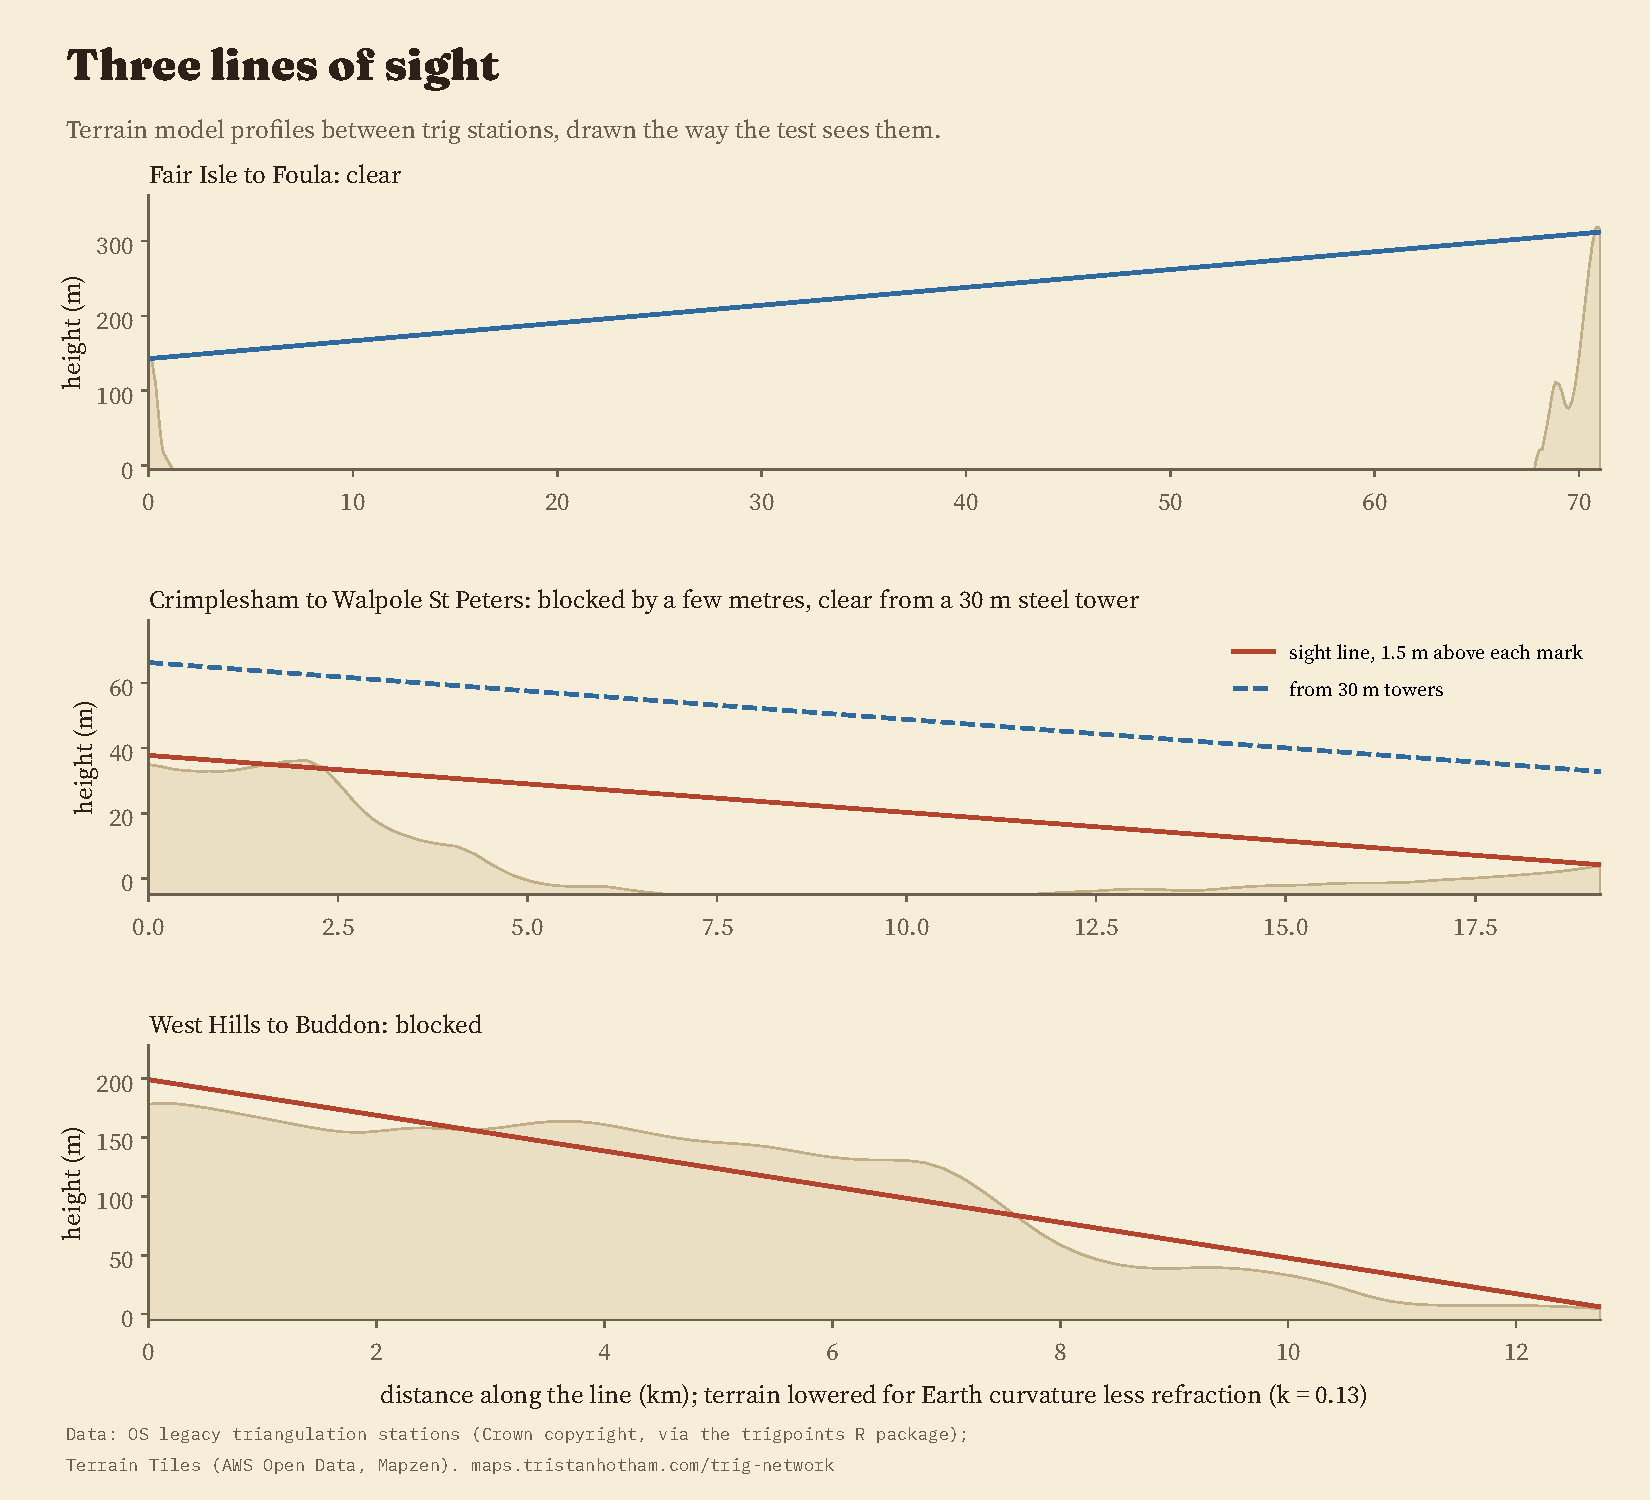
\includegraphics[width=\textwidth]{f_profiles.pdf}\caption{Three terrain profiles as the test sees them: a long clear sea crossing, a flat-country line blocked by a few metres and clear from 30 m towers, and a line to a ground mark blocked by rising ground.}\label{fig:profiles}\end{figure}

\subsection{Survival}
H5 is supported (Figure~\ref{fig:survival}; Appendix Table~\ref{tab:logit}). 415 of 6,573 pillars (6.3\%, CI 5.8 to 6.9) are recorded destroyed, against 26.1\% of intersected stations and 36.2\% of ground marks. In the planned logit (N = 24,421, 2,706 clusters), intersected stations have 3.25 times the odds of a pillar of being recorded destroyed (95\% CI 2.81 to 3.77) and ground marks 5.52 times (4.82 to 6.33). Lowland stations have 1.47 times the odds of upland ones (1.33 to 1.62). Secondary stations have lower odds than third-order ones (OR 0.64, 0.55 to 0.74); the primary estimate is similar but uncertain (0.68, 0.43 to 1.07). Scotland has lower odds than the South East (OR 0.70, 0.57 to 0.85); London does not differ clearly (0.95, 0.75 to 1.20). By region, the share of pillars recorded destroyed ranges from 2.3\% in Scotland to 13.6\% in Yorkshire and the Humber (Appendix Table~\ref{tab:region}).

\begin{figure}[tbp]\centering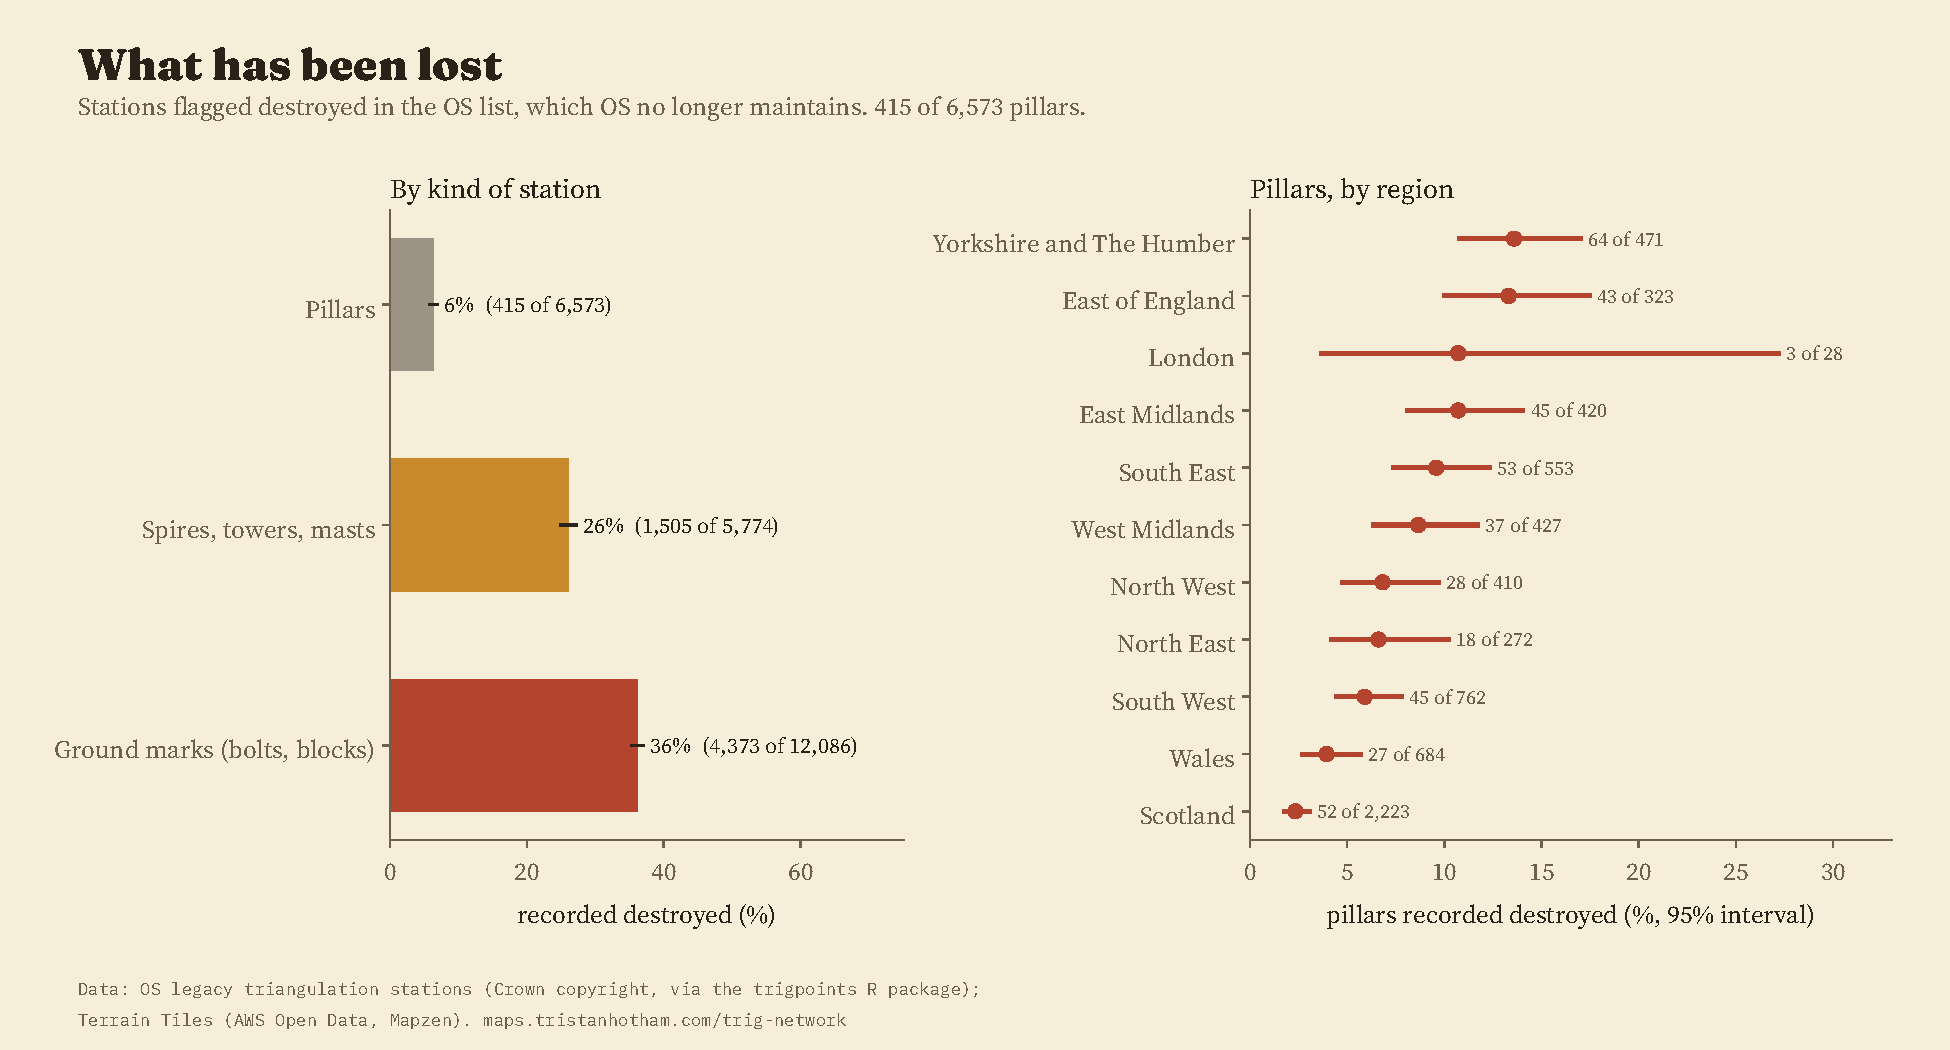
\includegraphics[width=\textwidth]{f_survival.pdf}\caption{Share recorded destroyed by kind of station, and for pillars by region, with Wilson 95\% intervals.}\label{fig:survival}\end{figure}

The OSM check points the same way: 29.1\% of the pillars not recorded destroyed have an OSM survey point within 50 m, against 2.9\% of those recorded destroyed (28.2\% and 2.9\% within 25 m; 29.5\% and 3.6\% within 100 m). For the 1,046 matched points with an elevation tag and a recorded OS height, the median absolute difference is 0.14 m, which suggests that many OSM elevations were copied from the OS list.

\section{Robustness and validation}\label{sec:robust}
\subsection{Planned robustness checks}
The intervisibility result is insensitive to the refraction coefficient over these distances: 95.0\% with no refraction, 95.0\% with $k = 0.075$ and 94.6\% with $k = 0.20$ (Figure~\ref{fig:robust}, Table~\ref{tab:robust}). Removing the end margin gives 94.2\%, a 500 m margin 95.4\%, a 50 m profile step 94.6\%, and the two nearest neighbours 94.3\% of 453 lines. Leaving out one region at a time gives 93.2\% to 96.6\%. Instrument height matters more: 90.4\% with the eye at the mark, 97.5\% from a 5 m signal. Pillar-to-pillar lines are clear 98.3\% of the time (176 of 179); lines with an intersected station at one end only 70\% (7 of 10), as expected when the structure's height is missing.

\begin{figure}[tbp]\centering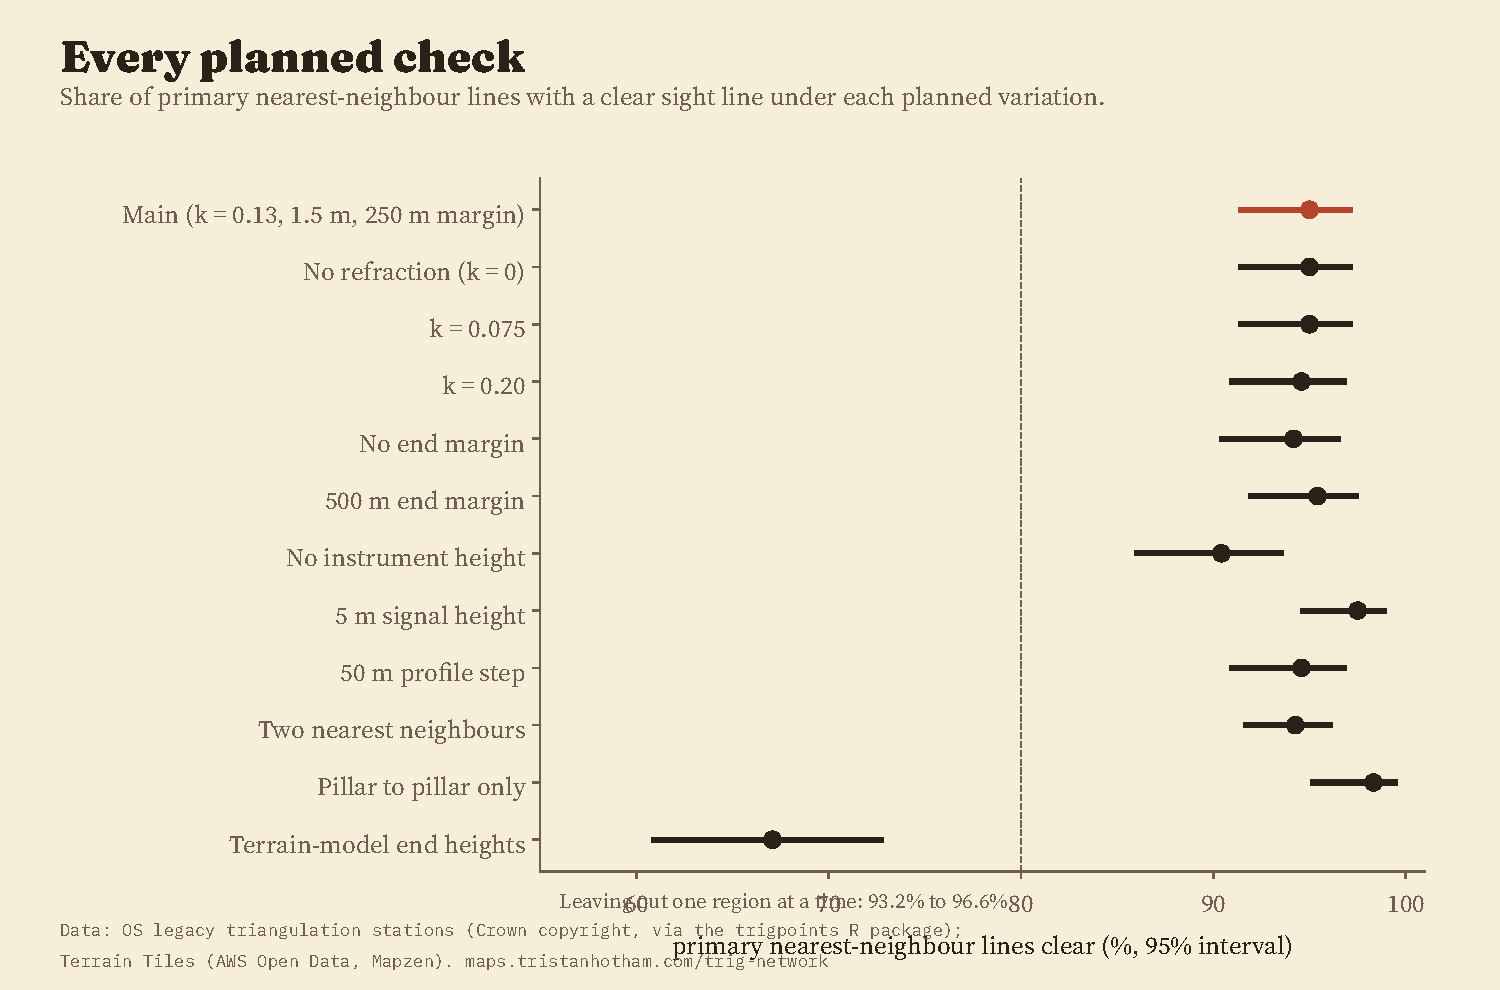
\includegraphics[width=0.85\textwidth]{f_robust.pdf}\caption{Every planned robustness check for the share of nearest-neighbour primary lines clear, with Wilson 95\% intervals.}\label{fig:robust}\end{figure}

\subsection{The terrain model and the surveyed heights}
One planned check changes the picture substantially. With the terrain model's own heights at both ends, only 67.1\% of primary lines are clear (CI 60.9 to 72.7). The reason is shown in Figure~\ref{fig:dem}: at 6,456 pillars with a recorded height, the terrain model is a median 22 m below the surveyed height (98.5\% are below), and the shortfall grows with height, from a few metres in the lowlands to about a hundred metres on the highest summits; for primary pillars the median is 34 m. A gap that grows with height points to smoothing rather than misregistration: at zoom 9 a pixel averages about 190 m of ground, and summits are the first thing lost, as resolution studies would predict \citep{zhang1994}. This matters for the interpretation of the placebos, whose ends sit on the smoothed terrain. A fair comparison uses terrain heights at both ends for the pillars too. On that basis, added after the main analysis and labelled exploratory, primary lines are still clear 50 percentage points more often than the 1 km shifted lines and 56 points more often than random land pairs.

\begin{figure}[tbp]\centering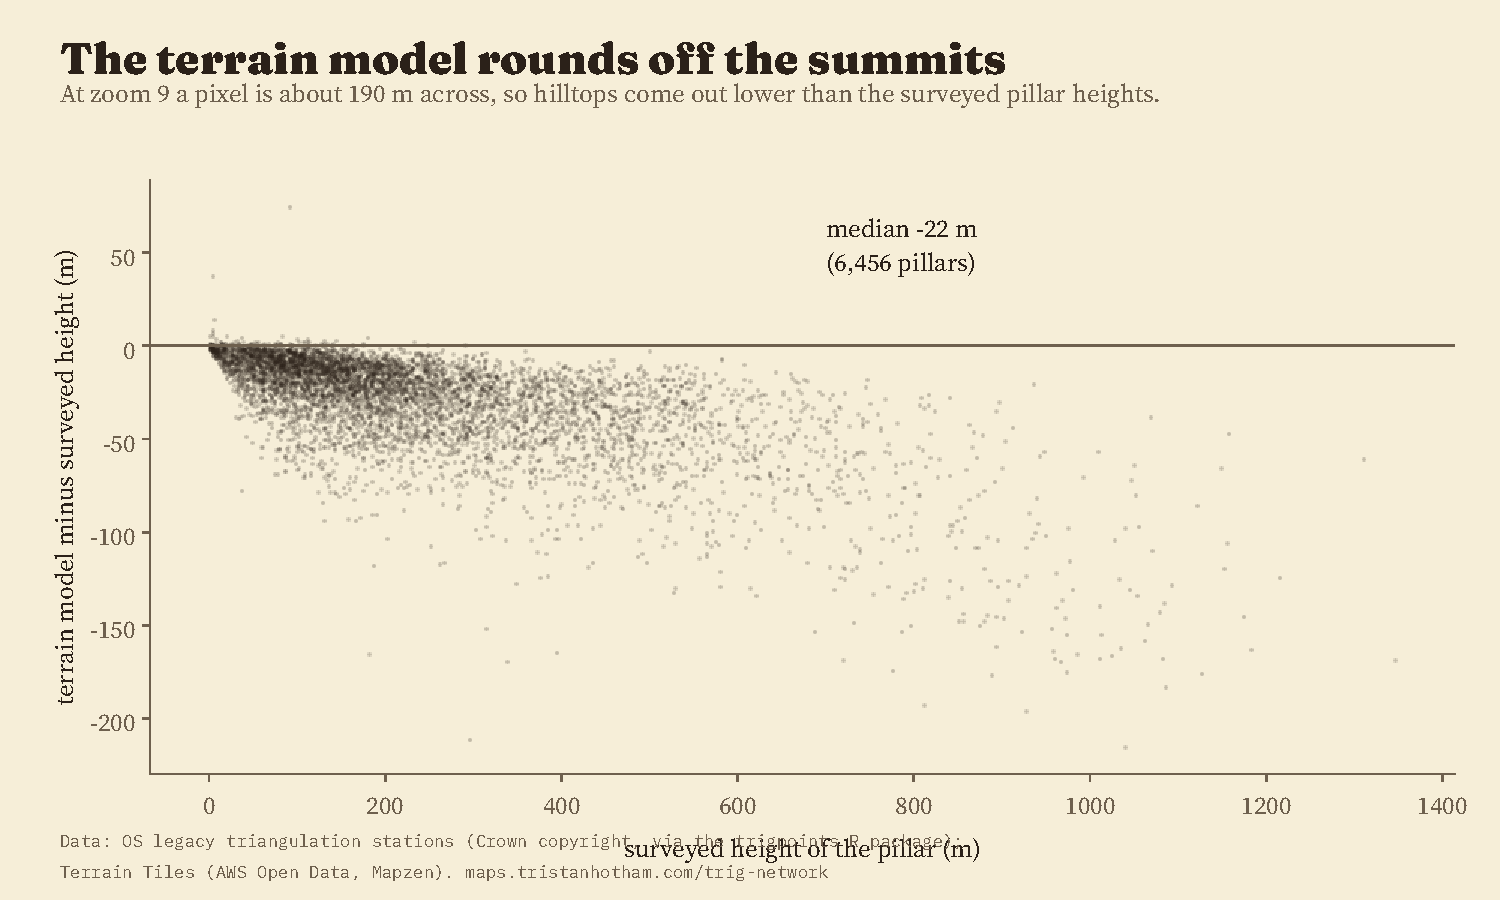
\includegraphics[width=0.85\textwidth]{f_dem.pdf}\caption{Terrain model height minus surveyed height at pillars with a recorded height.}\label{fig:dem}\end{figure}

\subsection{Survival model}
The lowland effect holds among pillars alone (OR 2.04, CI 1.59 to 2.61), with a 50 m threshold (1.33, 1.22 to 1.46) and without London (1.47); the intersected-station effect without London is 3.28 (2.83 to 3.81). Full estimates are in Appendix Table~\ref{tab:logit}.

\section{Discussion}\label{sec:disc}
\subsection{What the measurements show}
The legacy list reproduces the network the histories describe. Its orders nest, with each finer mesh at roughly a third of the spacing of the one above; its primary stations are far more regular than random points on the same land and form well-shaped triangles more often than random points would; and it was built, overwhelmingly, in the quarter century from 1936. None of this is surprising to a historian of the OS, but it is now measured, with uncertainty, from open data, and it gives a baseline for comparing other national networks.

The intervisibility result is the stronger finding. A coarse, open, global terrain model, with no trees or buildings and with summits rounded off by tens of metres, still confirms the design rule of the Retriangulation for 95\% of nearest-neighbour primary lines, once the surveyed station heights are used. The placebos show that this is not because British terrain is open: lines of the same lengths placed at random, or the same lines moved a kilometre, are mostly blocked. The surveyors' siting, the list's coordinates and heights, and the terrain model are mutually consistent. All but one of the failures are the expected ones. Structures such as spires and lighthouses were chosen precisely because they stand above the ground, and the list does not give their heights; and in the flat east, where lines at ground level were blocked by trees and buildings rather than terrain, the OS observed from towers, which the model also does not know about. That the only pillar-to-pillar failures fall at tower stations is a small but satisfying confirmation of the documentary record.

\subsection{Limitations}
First, nearest neighbours stand in for the lines actually observed. The list does not record which lines were observed, and the published diagrams of the Retriangulation \citep{os1967} were not used here; the Delaunay sides are a second proxy. Some nearest-neighbour pairs (for example two stations a few hundred metres apart at a base) may never have been observed. Second, the terrain model has no vegetation or buildings and its summits are too low; the main test leans on the list's heights, which are of the mark and not the ground, and may be ground or pillar-top heights in different cases. Third, the destroyed flag is out of date: the list is no longer maintained, so recorded destruction is a lower bound and its geography may partly reflect where the OS revisited stations. The TrigpointingUK database, which records condition from visits, lists 6,977 pillars of which 559 were logged as destroyed in 2025 \citep{tukpillar}, a different and broader count than the OS list's. Fourth, commissioning dates for primaries are block dates. Fifth, the analysis covers Great Britain only, as the list does; St Kilda lies outside the terrain tiles.

\subsection{Why the design shows so clearly}
It is worth asking why a terrain model with pixels nearly 200 m across can recover a design made with theodolites and lamps. Three features of the problem help. The lines are long (a median of 20.2 km for nearest primary neighbours), so the obstacles that matter are ridges and hills, which a coarse model captures, rather than hedges and buildings, which it does not. The stations sit on summits, where the line of sight leaves the station steeply downwards; the model's smoothing lowers the summit but also lowers the shoulders of the hill that might otherwise block the line near its ends, and the 250 m margin removes the first and last pixel from the test. And the surveyors were generous: the median primary line clears the terrain model by 27 m, so modest errors in either the model or the heights rarely change the verdict. Where clearances are small, in the flat east, the verdict does change, and there the documentary record says the surveyors needed towers.

The placebo comparison should be read with the terrain bias in mind. Placebo ends sit on the smoothed terrain, so they are lower than real ground on hilltops and the comparison flatters the pillars somewhat. The exploratory comparison with terrain-model heights at both ends removes that advantage, and the gap remains large. A sharper placebo, not attempted here, would move each station to the highest point within a given distance, asking whether the surveyors chose the best local summit or merely a good one; this is the siting problem studied by \citet{lee1991} and \citet{kim2004}, and the network could be used as a historical benchmark for siting algorithms.

\subsection{Implications}
For historians of surveying, the station list is a richer source than its gazetteer use suggests, and it can be checked against the terrain. For users of open terrain models, the comparison with surveyed pillar heights is a useful validation: thousands of precisely levelled points on summits, where models are weakest, show a systematic bias that grows with height. For heritage, the survival analysis gives a first quantitative picture of what has been lost, with the caveat that it rests on an unmaintained list. The pattern it shows is intuitive but now measured: marks on buildings and in the ground disappear with redevelopment, road works and farming, while pillars on open hilltops last. Lowland stations are more often lost, even among pillars, which is consistent with the pressures of farming and development, although the data cannot separate these causes. Linking the list to the condition reports of the TrigpointingUK community \citep{tukpillar}, which record visits rather than official revisions, would allow a much more current survival analysis and is an obvious next step.

\section{Conclusion}\label{sec:conc}
The Retriangulation of Great Britain can still be read from the OS legacy list and a modern terrain model. The network is a regular, nested mesh built in a generation; its pillars have outlasted its other marks; and its neighbouring primary stations are, in the terrain model, in sight of each other, unlike lines placed at random. This holds with the surveyed station heights at the ends; with the terrain model's own heights it holds for only 67\% of lines. All but one of the exceptions are structures and towers the model does not know about. The data and code released with the paper make the measurements reproducible and extendable, for example to the published observation diagrams, to higher-resolution terrain, or to other national networks.

\section*{Data availability statement}
Data and code: Zenodo DOI https://doi.org/10.5281/zenodo.24104644. The interactive map is at \url{https://maps.tristanhotham.com/trig-network/} and the repository at \url{https://github.com/Tristan-Hotham/trig-network}. The station list contains OS data \textcopyright\ Crown copyright and database right 2018, used under the Open Government Licence v3.0, via the trigpoints R package \citep{jones2018}; terrain from Terrain Tiles (AWS Open Data; Mapzen) \citep{tilezen}; OpenStreetMap data \textcopyright\ OpenStreetMap contributors (ODbL); region boundaries from the Office for National Statistics (Open Government Licence v3.0).

\section*{AI statement}
I wrote the text, with drafting and editing assistance from Claude (Anthropic), which also helped prepare the analysis code. I reviewed and checked all text and results.

\begin{thebibliography}{99}
\bibitem[Amante and Eakins(2009)]{amante2009} Amante, C. and Eakins, B. W. (2009) \textit{ETOPO1 1 Arc-Minute Global Relief Model: Procedures, Data Sources and Analysis}. NOAA Technical Memorandum NESDIS NGDC-24. Boulder: National Geophysical Data Center. doi:10.7289/V5C8276M.
\bibitem[Ashkenazi et al.(1972)]{ashkenazi1972} Ashkenazi, V., Cross, P. A., Davies, M. J. K. and Proctor, D. W. (1972) \textit{The Readjustment of the Retriangulation of Great Britain, and its Relationship to the European Terrestrial and Satellite Networks}. Ordnance Survey Professional Papers, New Series, 24. Southampton: Ordnance Survey.
\bibitem[Ashkenazi et al.(1983)]{ashkenazi1983} Ashkenazi, V., Crane, A. S., Preiss, W. J. and Williams, J. W. (1983) \textit{The 1980 Readjustment of the Triangulation of the United Kingdom and the Republic of Ireland, OS(SN)80}. Ordnance Survey Professional Paper, New Series, 31. Southampton: Ordnance Survey.
\bibitem[Baddeley et al.(2015)]{baddeley2015} Baddeley, A., Rubak, E. and Turner, R. (2015) \textit{Spatial Point Patterns: Methodology and Applications with R}. Boca Raton: CRC Press.
\bibitem[Barber et al.(1996)]{barber1996} Barber, C. B., Dobkin, D. P. and Huhdanpaa, H. (1996) The Quickhull algorithm for convex hulls. \textit{ACM Transactions on Mathematical Software} 22(4), 469 to 483. doi:10.1145/235815.235821.
\bibitem[Cameron and Miller(2015)]{cameron2015} Cameron, A. C. and Miller, D. L. (2015) A practitioner's guide to cluster-robust inference. \textit{Journal of Human Resources} 50(2), 317 to 372.
\bibitem[Clark and Evans(1954)]{clarkevans1954} Clark, P. J. and Evans, F. C. (1954) Distance to nearest neighbor as a measure of spatial relationships in populations. \textit{Ecology} 35(4), 445 to 453. doi:10.2307/1931034.
\bibitem[Clarke(1858)]{clarke1858} Clarke, A. R. (1858) \textit{Account of the Observations and Calculation of the Principal Triangulation and of the Figure, Dimensions and Mean Specific Gravity of the Earth as Derived Therefrom}. London: Eyre and Spottiswoode.
\bibitem[Danielson and Gesch(2011)]{danielson2011} Danielson, J. J. and Gesch, D. B. (2011) \textit{Global Multi-Resolution Terrain Elevation Data 2010 (GMTED2010)}. U.S. Geological Survey Open-File Report 2011-1073. doi:10.3133/ofr20111073.
\bibitem[De Floriani and Magillo(1994)]{defloriani1994} De Floriani, L. and Magillo, P. (1994) Visibility algorithms on triangulated digital terrain models. \textit{International Journal of Geographical Information Systems} 8(1), 13 to 41. doi:10.1080/02693799408901985.
\bibitem[Delaunay(1934)]{delaunay1934} Delaunay, B. (1934) Sur la sph\`ere vide. \textit{Bulletin de l'Acad\'emie des Sciences de l'URSS, Classe des sciences math\'ematiques et naturelles} no. 6, 793 to 800.
\bibitem[Edney(1997)]{edney1997} Edney, M. H. (1997) \textit{Mapping an Empire: The Geographical Construction of British India, 1765 to 1843}. Chicago: University of Chicago Press.
\bibitem[Efron(1979)]{efron1979} Efron, B. (1979) Bootstrap methods: another look at the jackknife. \textit{Annals of Statistics} 7(1), 1 to 26.
\bibitem[Farr et al.(2007)]{farr2007} Farr, T. G. et al. (2007) The Shuttle Radar Topography Mission. \textit{Reviews of Geophysics} 45(2), RG2004. doi:10.1029/2005RG000183.
\bibitem[Fisher(1991)]{fisher1991} Fisher, P. F. (1991) First experiments in viewshed uncertainty: the accuracy of the viewshed area. \textit{Photogrammetric Engineering and Remote Sensing} 57(10), 1321 to 1327.
\bibitem[Fisher(1993)]{fisher1993} Fisher, P. F. (1993) Algorithm and implementation uncertainty in viewshed analysis. \textit{International Journal of Geographical Information Systems} 7(4), 331 to 347. doi:10.1080/02693799308901965.
\bibitem[Greaves(2004)]{greaves2004} Greaves, M. (2004) OSTN02: a new definitive transformation from GPS derived coordinates to National Grid coordinates in Great Britain. \textit{Survey Review} 37(293), 502 to 519.
\bibitem[Hewitt(2010)]{hewitt2010} Hewitt, R. (2010) \textit{Map of a Nation: A Biography of the Ordnance Survey}. London: Granta.
\bibitem[Hirt et al.(2010)]{hirt2010} Hirt, C., Guillaume, S., Wisbar, A., B\"urki, B. and Sternberg, H. (2010) Monitoring of the refraction coefficient in the lower atmosphere using a controlled setup of simultaneous reciprocal vertical angle measurements. \textit{Journal of Geophysical Research: Atmospheres} 115, D21102. doi:10.1029/2010JD014067.
\bibitem[Jones(2018)]{jones2018} Jones, P. M. (2018) \textit{trigpoints: Data Set of Trig Points in Great Britain in British National Grid Coordinates}. R package version 1.0.0, MIT licence. Contains OS data \textcopyright\ Crown copyright and database right 2018. \url{https://github.com/philmikejones/trigpoints}.
\bibitem[Kim et al.(2004)]{kim2004} Kim, Y.-H., Rana, S. and Wise, S. (2004) Exploring multiple viewshed analysis using terrain features and optimisation techniques. \textit{Computers and Geosciences} 30(9 to 10), 1019 to 1032. doi:10.1016/j.cageo.2004.07.008.
\bibitem[Lee(1991)]{lee1991} Lee, J. (1991) Analyses of visibility sites on topographic surfaces. \textit{International Journal of Geographical Information Systems} 5(4), 413 to 429. doi:10.1080/02693799108927866.
\bibitem[Ordnance Survey(1967)]{os1967} Ordnance Survey (1967) \textit{The History of the Retriangulation of Great Britain 1935 to 1962}. London: HMSO.
\bibitem[Ordnance Survey(2016)]{osblog2016} Ordnance Survey (2016) History of the trig pillar. Ordnance Survey blog, 19 April 2016. \url{https://www.ordnancesurvey.co.uk/blog/a-history-of-the-trig-pillar}.
\bibitem[Owen and Pilbeam(1992)]{owen1992} Owen, T. and Pilbeam, E. (1992) \textit{Ordnance Survey: Map Makers to Britain since 1791}. Southampton: Ordnance Survey; London: HMSO.
\bibitem[Ripley(1977)]{ripley1977} Ripley, B. D. (1977) Modelling spatial patterns. \textit{Journal of the Royal Statistical Society, Series B} 39(2), 172 to 192. doi:10.1111/j.2517-6161.1977.tb01615.x.
\bibitem[Roy(1790)]{roy1790} Roy, W. (1790) An account of the trigonometrical operation, whereby the distance between the meridians of the Royal Observatories of Greenwich and Paris has been determined. \textit{Philosophical Transactions of the Royal Society of London} 80. JSTOR 106834.
\bibitem[Seabold and Perktold(2010)]{seabold2010} Seabold, S. and Perktold, J. (2010) statsmodels: econometric and statistical modeling with Python. \textit{Proceedings of the 9th Python in Science Conference}.
\bibitem[Seymour(1980)]{seymour1980} Seymour, W. A. (ed.) (1980) \textit{A History of the Ordnance Survey}. Folkestone: Dawson.
\bibitem[Tilezen(n.d.)]{tilezen} Tilezen (n.d.) Joerd documentation: data sources and attribution for Terrain Tiles. \url{https://github.com/tilezen/joerd/blob/master/docs/data-sources.md}, retrieved 2026.
\bibitem[TrigpointingUK(2026a)]{tukbilby} TrigpointingUK (2026a) Bilby towers. TrigpointingUK wiki. \url{https://wiki.trigpointing.uk/Bilby_towers}, retrieved 2026.
\bibitem[TrigpointingUK(2026b)]{tukpillar} TrigpointingUK (2026b) Pillar. TrigpointingUK wiki. \url{https://wiki.trigpointing.uk/Pillar}, retrieved 2026.
\bibitem[Virtanen et al.(2020)]{virtanen2020} Virtanen, P. et al. (2020) SciPy 1.0: fundamental algorithms for scientific computing in Python. \textit{Nature Methods} 17, 261 to 272. doi:10.1038/s41592-019-0686-2.
\bibitem[Wilson(1927)]{wilson1927} Wilson, E. B. (1927) Probable inference, the law of succession, and statistical inference. \textit{Journal of the American Statistical Association} 22(158), 209 to 212. doi:10.2307/2276774.
\bibitem[Zhang and Montgomery(1994)]{zhang1994} Zhang, W. and Montgomery, D. R. (1994) Digital elevation model grid size, landscape representation, and hydrologic simulations. \textit{Water Resources Research} 30(4), 1019 to 1028. doi:10.1029/93WR03553.
\end{thebibliography}

\appendix
\section{Data construction details}\label{app:data}
{\raggedright\textbf{Kinds of station.} Pillar: any row of type PILLAR. Ground marks: BOLT, RIVET, BLOCK, BURIED BLK, CENTRE, DISC, CUT, HOLE, PEG, PLATE, PUNCH MARK, MARK, SPIDER, FENOMARK, CURRY ST'L, PIPE, POST, STONE, CAIRN, OLD TRIG. Intersected or roof stations: SPIRE, FLAGSTAFF, VANE, CHIMNEY, MAST, LIGHTHOUSE, CUPOLA, DOME, BELFRY, TOWER, PINNACLE, BEACON, CROSS, APEX, AERIAL, L'NING C, MONUMENT, OBELISK, MEMORIAL, TURRET, VENT, LAMP, POLE, PYLON, WIRE, HYDROG, TOPOGRAPH.\par}

\textbf{Dates.} com\_date is a count of days since 1 January 1970; one value in 2052 and values outside 1930 to 2000 were treated as missing. A station's year is the earliest among its rows.

\textbf{Steel tower stations.} The 22 primary stations listed on the TrigpointingUK wiki page ``Bilby towers'' (which cites section 2.07 of the official history) are listed in code/steel\_towers.csv; all 22 match a primary station of the same name in the list.

\textbf{OSM.} Survey points were matched to the nearest OS station; three polygon geometries (Irish baseline towers) take their first vertex.

\begin{table}[tbp]\centering\scriptsize\caption{Planned logit of the destroyed flag, all stations with a terrain value and a commissioning decade. Standard errors clustered by 10 km grid square. N = 24,421; clusters = 2,706; pseudo-$R^2$ = 0.125.}\label{tab:logit}\begin{tabular}{p{7.2cm}rrlr}\toprule Term & Coef. & (SE) & OR [95\% CI] & $p$\\\midrule
Intercept & $-$2.829 & (0.088) & 0.06 [0.05, 0.07] & 0.000\\
Kind: intersected (vs pillar) & 1.180 & (0.075) & 3.25 [2.81, 3.77] & 0.000\\
Kind: surface (vs pillar) & 1.709 & (0.070) & 5.52 [4.82, 6.33] & 0.000\\
Order: 1 (vs 3) & $-$0.390 & (0.235) & 0.68 [0.43, 1.07] & 0.097\\
Order: 2 (vs 3) & $-$0.447 & (0.076) & 0.64 [0.55, 0.74] & 0.000\\
Order: 4 (vs 3) & 0.604 & (0.051) & 1.83 [1.65, 2.02] & 0.000\\
Order: other (vs 3) & $-$0.873 & (0.352) & 0.42 [0.21, 0.83] & 0.013\\
Region: East Midlands (vs South East) & $-$0.124 & (0.094) & 0.88 [0.73, 1.06] & 0.187\\
Region: East of England (vs South East) & $-$0.045 & (0.083) & 0.96 [0.81, 1.12] & 0.585\\
Region: London (vs South East) & $-$0.056 & (0.120) & 0.95 [0.75, 1.20] & 0.643\\
Region: North East (vs South East) & 0.543 & (0.104) & 1.72 [1.40, 2.11] & 0.000\\
Region: North West (vs South East) & $-$0.062 & (0.092) & 0.94 [0.78, 1.13] & 0.498\\
Region: Scotland (vs South East) & $-$0.360 & (0.099) & 0.70 [0.57, 0.85] & 0.000\\
Region: South West (vs South East) & $-$0.174 & (0.091) & 0.84 [0.70, 1.01] & 0.057\\
Region: Wales (vs South East) & $-$0.205 & (0.094) & 0.81 [0.68, 0.98] & 0.030\\
Region: West Midlands (vs South East) & 0.066 & (0.100) & 1.07 [0.88, 1.30] & 0.509\\
Region: Yorkshire and The Humber (vs South East) & 0.071 & (0.094) & 1.07 [0.89, 1.29] & 0.447\\
Decade: 1930s (vs 1950s) & 0.451 & (0.131) & 1.57 [1.22, 2.03] & 0.001\\
Decade: 1940s (vs 1950s) & 0.470 & (0.047) & 1.60 [1.46, 1.75] & 0.000\\
Decade: 1960 on (vs 1950s) & $-$0.768 & (0.069) & 0.46 [0.41, 0.53] & 0.000\\
Lowland (below 100 m) & 0.384 & (0.050) & 1.47 [1.33, 1.62] & 0.000\\
\bottomrule\end{tabular}\end{table}

\begin{table}[tbp]\centering\small\caption{Stations and pillars recorded destroyed by region.}\label{tab:region}\begin{tabular}{lrrrrr}\toprule Region & Stations & Destroyed (\%) & Pillars & Destroyed & (\%)\\\midrule
Scotland & 4,653 & 14.9 & 2,223 & 52 & 2.3\\
Wales & 2,002 & 22.6 & 684 & 27 & 3.9\\
South West & 2,623 & 24.1 & 762 & 45 & 5.9\\
North East & 978 & 37.3 & 272 & 18 & 6.6\\
North West & 2,129 & 29.9 & 410 & 28 & 6.8\\
West Midlands & 1,771 & 30.0 & 427 & 37 & 8.7\\
South East & 3,272 & 31.0 & 553 & 53 & 9.6\\
East Midlands & 1,967 & 24.8 & 420 & 45 & 10.7\\
London & 795 & 34.3 & 28 & 3 & 10.7\\
East of England & 2,202 & 28.4 & 323 & 43 & 13.3\\
Yorkshire and The Humber & 2,041 & 28.5 & 471 & 64 & 13.6\\
\bottomrule\end{tabular}\end{table}

\begin{table}[tbp]\centering\small\caption{Planned robustness checks for nearest-neighbour primary lines (Wilson 95\% CI).}\label{tab:robust}\begin{tabular}{lrrl}\toprule Check & Clear & Lines & \% clear [95\% CI]\\\midrule
Main ($k = 0.13$, 1.5 m, 250 m margin, 100 m step) & 228 & 240 & 95.0 [91.5, 97.1]\\
$k = 0$ & 228 & 240 & 95.0 [91.5, 97.1]\\
$k = 0.075$ & 228 & 240 & 95.0 [91.5, 97.1]\\
$k = 0.20$ & 227 & 240 & 94.6 [91.0, 96.8]\\
No end margin & 226 & 240 & 94.2 [90.4, 96.5]\\
500 m end margin & 229 & 240 & 95.4 [92.0, 97.4]\\
Instrument height 0 m & 217 & 240 & 90.4 [86.0, 93.5]\\
Signal height 5 m & 234 & 240 & 97.5 [94.7, 98.8]\\
50 m profile step & 227 & 240 & 94.6 [91.0, 96.8]\\
Two nearest neighbours & 427 & 453 & 94.3 [91.7, 96.1]\\
Pillar to pillar only & 176 & 179 & 98.3 [95.2, 99.4]\\
Any intersected station & 7 & 10 & 70.0 [39.7, 89.2]\\
Terrain-model heights at the ends & 161 & 240 & 67.1 [60.9, 72.7]\\
\midrule\multicolumn{4}{l}{\textit{Leave one region out (\% clear)}}\\
\quad without East Midlands & & & 95.5\\
\quad without East of England & & & 96.6\\
\quad without London & & & 95.4\\
\quad without North East & & & 94.9\\
\quad without North West & & & 94.7\\
\quad without Scotland & & & 93.2\\
\quad without South East & & & 95.0\\
\quad without South West & & & 95.2\\
\quad without Wales & & & 94.5\\
\quad without West Midlands & & & 94.8\\
\quad without Yorkshire and The Humber & & & 94.7\\
\bottomrule\end{tabular}\end{table}

\end{document}
